\chapter{Machine Learning Theory} \label{chap:ml}

This section will act as a theory section for the machine learning models used. Machine learning models are a subset of artificial intelligence models. Machine learning models extract rules from data, which can then be applied to classify, or estimate components of another dataset called the \textit{target variable}. What makes machine learning models different from other artificial intelligence models, is that the rules for making predictions on the target variable are not given to the model explicitly. Instead, the models are given data and subsequently extract the rules for making predictions themselves. Machine learning algorithms are formally divided into \textit{supervised learning}, \textit{unsupervised learning} and \textit{semi-supervised learning}. Supervised learning models require labeled datasets to extract information from the dataset, and are usually used to perform classification or regression tasks. Unsupervised learning algorithms do not require labeled datasets. There also exist hybrid models called \textit{semi-supervised learning} that use a combination of labeled and unlabelled datasets. Two sections of this chapter are dedicated to the two most central machine learning models encountered in this work; clustering and \acrshort{ann}. Section \ref{sec:theory_clust} will give the theoretical background of the similarity measures, and the clustering algorithm used. Section \ref{sec:ann} will explain the basic building blocks of \acrshort{ann}, the different layers in a \acrshort{ann}, and how they are trained. In the paragraph below, the definition of a time series is given, which is the definition that is used throughout this work. \bigskip

\subsection*{What Is a Time Series?}
A time series is defined as a set of observations $\{x_t\}$ recorded at a specific time $t$. A discrete-time series is a time series where the set of times when observations are made ($T_0$) is discrete \cite{brockwell_davis_advanced}. A multivariate time series can be viewed as a set of vectors $\{\mathbf{x}_t\}$ where each set of vector elements $\{x^i_t\}$ is an individual time series. This means that the elements of the same vector $[x^1_t, x^2_t,...,x^N_t]$ are separate observations. A \acrshort{gls} curve extracted from an ultrasound video from the \acrshort{4ch} view of a patient can be considered a univariate time series. In contrast, the \acrshort{gls} curves extracted from the ultrasound videos of all the three views for a single patient can be considered a multivariate time series. \bigskip

\section{Clustering} \label{sec:theory_clust}
There are three types of \acrfull{tsc}, \textit{whole-series \acrshort{tsc}}, \textit{subsequence \acrshort{tsc}} and \textit{time-point \acrshort{tsc}}. Whole-series \acrshort{tsc} is when multiple ''whole'' time series are clustered with respect to each other. Subsequence \acrshort{tsc} comprises the clustering of subsequences of the same time series with respect to each other. The defining difference between whole-series and subsequence \acrshort{tsc} is that whole-series \acrshort{tsc} clusters multiple time series while subsequence \acrshort{tsc} clusters different subsequences of the same time series. When performing time-point \acrshort{tsc} the goal is to cluster individual observations of a time series with regard to to each other. In this review we will only consider work using whole-series \acrshort{tsc}, so when the phrase \textit{time-series clustering} is used, one can assume that whole-series \acrshort{tsc} is what is being referred to. \bigskip

Whole series \acrshort{tsc} can broadly be divided into three main approaches: the raw-data based approach, the feature-based approach, and the model-based approach. In the raw-data based approach, one measures the similarity between the raw time series themselves and clusters them based on this. When clustering raw time series, the majority of the work goes into the selection of similarity metric and clustering algorithm, and one clusters the time series with regard to similarity in time or similarity in shape \cite{tsc_rev}. In the feature-based approach, one also clusters time series with regard to similarity in time and shape, but the work is somewhat shifted away from the choice of similarity metric and over to the choice of representation. Either to extract more relevant information from the time series or to reduce the computational complexity of the similarity measurement. In the model-based approach, the goal is most often to cluster time series with regard to the underlying data generating process \cite{moar_mpl_tsc}. The underlying assumption being that two time series that appear different, might still have been generated by the same process.

\begin{figure}
    \begin{center}
    \tikzstyle{int} = [pin edge={to-,thin,black}]
\tikzstyle{sqr}  = [rectangle, rounded corners, minimum width=4.25cm, minimum height=1cm,text centered, draw=black, fill=white]
\tikzstyle{arrow} = [thin,->,>=stealth]

\begin{tikzpicture}[node distance=1.75cm]

%% Model-based approach
\node (inp_mod) [int] {Raw time series};
\node (rep_mod) [sqr, below of=inp_mod] {Model parameters};
\node (sim_mod) [sqr, below of=rep_mod] {Similarity measurement};
\node (clu_mod) [sqr, below of=sim_mod] {Clustering};
\node (out_mod) [int, below of=clu_mod] {Cluster assignments};

%% Feature-based approach
\node (inp_fea) [int, right of=inp_mod, xshift=3cm] {Raw time series};
\node (rep_fea) [sqr, below of=inp_fea] {Extracted features};
\node (sim_fea) [sqr, below of=rep_fea] {Similarity measurement};
\node (clu_fea) [sqr, below of=sim_fea] {Clustering};
\node (out_fea) [int, below of=clu_fea] {Clusters assignments};

%% Raw-data based approach
\node (inp_raw) [int, right of=inp_fea, xshift=3cm] {Raw time series};
\node (sim_raw) [sqr, right of=sim_fea, xshift=3cm] {Similarity measurement};
\node (clu_raw) [sqr, below of=sim_raw] {Clustering};
\node (out_raw) [int, below of=clu_raw] {Clusters assignments};

%% Names
\node (nam_mod) [int, below of=out_mod, yshift=1cm] {\textbf{(Model-based)}};
\node (nam_fea) [int, below of=out_fea, yshift=1cm] {\textbf{(Feature-based)}};
\node (nam_raw) [int, below of=out_raw, yshift=1cm] {\textbf{(Raw-data based)}};

%% Arrows
\draw [arrow] (inp_mod) -- (rep_mod);
\draw [arrow] (rep_mod) -- (sim_mod);
\draw [arrow] (sim_mod) -- (clu_mod);
\draw [arrow] (clu_mod) -- (out_mod);

\draw [arrow] (inp_fea) -- (rep_fea);
\draw [arrow] (rep_fea) -- (sim_fea);
\draw [arrow] (sim_fea) -- (clu_fea);
\draw [arrow] (clu_fea) -- (out_fea);

\draw [arrow] (inp_raw) -- (sim_raw);
\draw [arrow] (sim_raw) -- (clu_raw);
\draw [arrow] (clu_raw) -- (out_raw);
\end{tikzpicture}
    \end{center}
    \caption{Illustration of the three approaches to whole-series \acrshort{tsc}, and their components. The illustration is inspired by figure 2 in \textcite{tsc_rev}.}
    \label{fig:tsc_approaches}
\end{figure}

The common denominator of the three approaches to \acrshort{tsc} mentioned is that they are all made up of three distinct parts: representation method, similarity measurement, and clustering algorithm. This is illustrated in figure \ref{fig:tsc_approaches}. Another key aspect of the \acrshort{tsc} model is what the \textbf{objective} is. It is broadly considered to be three objectives one can cluster with regard to: similarity in time, similarity in shape, and similarity in change \cite{tsc_rev}. When calculating the similarity between all combinations of time series, the resulting similarity metric is stored in what is called a \textit{dissimilarity matrix}. The choice of similarity metric is important in a raw-data approach as it decides which aspects of the time series will be used to measure (dis)similarity. It has a significant impact on the time-complexity of the clustering system. \acrshort{pvc} has a similar approach as raw-data based \acrshort{tsc}, the dissimilarities between data points are measured, and are passed on to the clustering algorithm. In the subsection below, the dissimilarity measures used in the clustering models of this work are described.

\subsection{Dissimilarity Metric} \label{sec:theory_diss}
When clustering point-values, the choice of metric used to measure dissimilarity between the data objects are usually some sort of distance measure. The choices of distance measures are varied and plentiful. Options include: Euclidean distance, Manhattan distance, and Minkowski distance. In the \acrshort{pvc} models, the Euclidean distance is used because it is the easiest to interpret geometrically. It is defined in equation \eqref{eq:ed} for two data objects $x$, and $y$ of $N$ dimensions.

\begin{equation}
    ED(x,y) = \sqrt{\sum_{i = 1}^N (x_i - y_i)^2}
    \label{eq:ed}
\end{equation}

\begin{figure}
    \centering
    \begin{subfigure}[b]{0.49\textwidth}
        \centering
        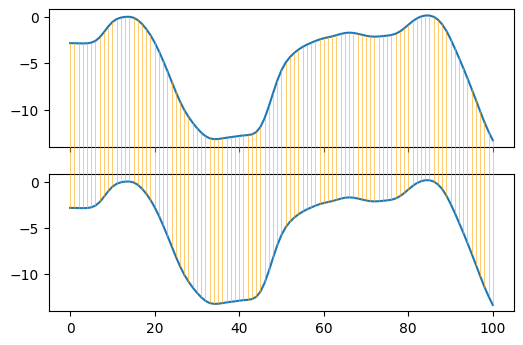
\includegraphics[width=0.99\textwidth]{machine-learning/warping_lines_1_curve.png}
        \caption{Sample-wise Euclidean distance.}
        \label{fig:ed_ex}
    \end{subfigure}
    \begin{subfigure}[b]{0.49\textwidth}
        \centering
        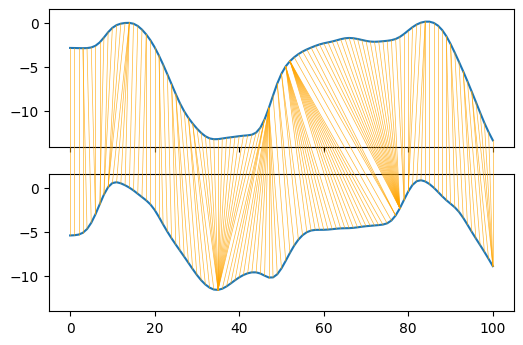
\includegraphics[width=0.99\textwidth]{machine-learning/warping_lines_2_curves.png}
        \caption{\acrshort{dtw} distance.}
        \label{fig:dtw_ex}
    \end{subfigure}
    \caption{An illustration of the difference between sample-wise Euclidean distance between time series, and \acrshort{dtw} distance between time series.}
    \label{fig:ed_dtw_ex}
\end{figure}

In the raw-data based approach to \acrshort{tsc}, choice of dissimilarity metric is paramount and is chosen based on what objective of the \acrshort{tsc} is, and the different lengths of the time series to be compared. When clustering with regard to similarity in shape, the similarity metric can be lock-step (one-to-one) or elastic (one-to-many) \cite{tsc_rev}. An example of a lock-step measure is the use of Euclidean distance to measure the distance between time series sample-wise. However, this becomes problematic when the time series are not of equal length. \acrfull{dtw} distance is a powerful alternative for Euclidean distance to measure the shape-based distance between two time series. To understand how the \acrshort{dtw} distance works as a dissimilarity metric, one can imagine that it warps one time series such that the two series are equal in length, and then measures the Euclidean distance between them. This is illustrated in figure \ref{fig:ed_dtw_ex}. \acrshort{dtw} is probably most famous from speech recognition, where it is applied to find out which phoneme\footnote{Phoneme is a term from speech recognition and refers to the largest unit of sound for which the frequency spectrum is constant. Phonemes are considered as the ''atomic sounds'' that make up speech.} in a dictionary of phonemes is the optimal fit to a recorded sound. To calculate the \acrshort{dtw} distance between two time series $x$ and $y$ of length $n$ and $m$ respectively. First an $(n \times m)$ matrix is constructed called the \acrfull{lcm}. Element $\mathrm{LCM}(i,j)$ is the sample-wise quadratic distance between $x_i$ and $y_i$ ($(x_i - y_i)^2$). The next step is to create a warping path $P = \{p_1, p_2, ..., p_L\}$ across the \acrshort{lcm}. The warping path must fulfill three conditions: the boundary condition, the continuity condition, and the monotonicity condition. 

\begin{enumerate} 
    \item \textbf{Boundary}: The path must begin and end in the corners of the \acrshort{lcm}. $p_0 = \mathrm{LCM(1,1)}$, $p_L = \mathrm{LCM(n,m)}$ 
    \item \textbf{Continuity}: Two adjacent warping steps $p_k$ and $p_{k+1}$ must be equal to adjacent elements on the \acrshort{lcm}. This means that the matrix elements that $p_k$ and $p_{k+1}$ point to, must be adjacent horizontally, vertically or diagonally in the \acrshort{lcm}.
    \item \textbf{Monotonicity}: The warping path must increase monotonically. This means that the warping path cannot go backwards index-wise. If one combines the continuity, and monotonicity constraints, and lets $p_k = \mathrm{LCM}(i,j)$, valid values for $p_k$ are $\mathrm{LCM}(i+1,j)$, $\mathrm{LCM}(i,j+1)$ and $\mathrm{LCM}(i+1,j+1)$.
\end{enumerate}

The warping distance of the warping path $P$ is the sum of the \acrshort{lcm} elements that entries of $P$ are equal to. The \acrshort{dtw} distance between time series $x$ and $y$ is then defined as the square root of the smallest possible warping distance between $x$ and $y$. The warping path corresponding to the smallest warping distance can be found by using a recurrent algorithm from dynamic programming shown in equation \eqref{eq:dp_dtw} \cite{pjotr}.

\begin{equation}
    \begin{split}
        p_1     &= \mathrm{LCM}\{ 1,1 \}, p_L = \mathrm{LCM}\{ n,m \}  \\
        p_{i}   &= \mathrm{LCM}\{ f,g \} \\
        p_{i+1} &= \mathrm{min} \left \{ \mathrm{LCM} \{ f+1,g\}, \mathrm{LCM} \{ f,g+1\}, \mathrm{LCM} \{ f+1,g+1\} \right  \}
    \end{split}
    \label{eq:dp_dtw}
\end{equation}

Although the \acrshort{dtw} distance is more flexible than estimating Euclidean distance between two time series, it comes at the cost of much higher run time and space requirements. The time complexity for calculating the dissimilarity matrix of a set of $N$ time series using the \acrshort{dtw} distance is $O\left ( n m N^{2} \right )$ \cite{tsc_rev}. An illustration of how the \acrshort{dtw} distance between two time series is estimated is shown in figure \ref{fig:warping_path}. 

\begin{figure}
    \centering
    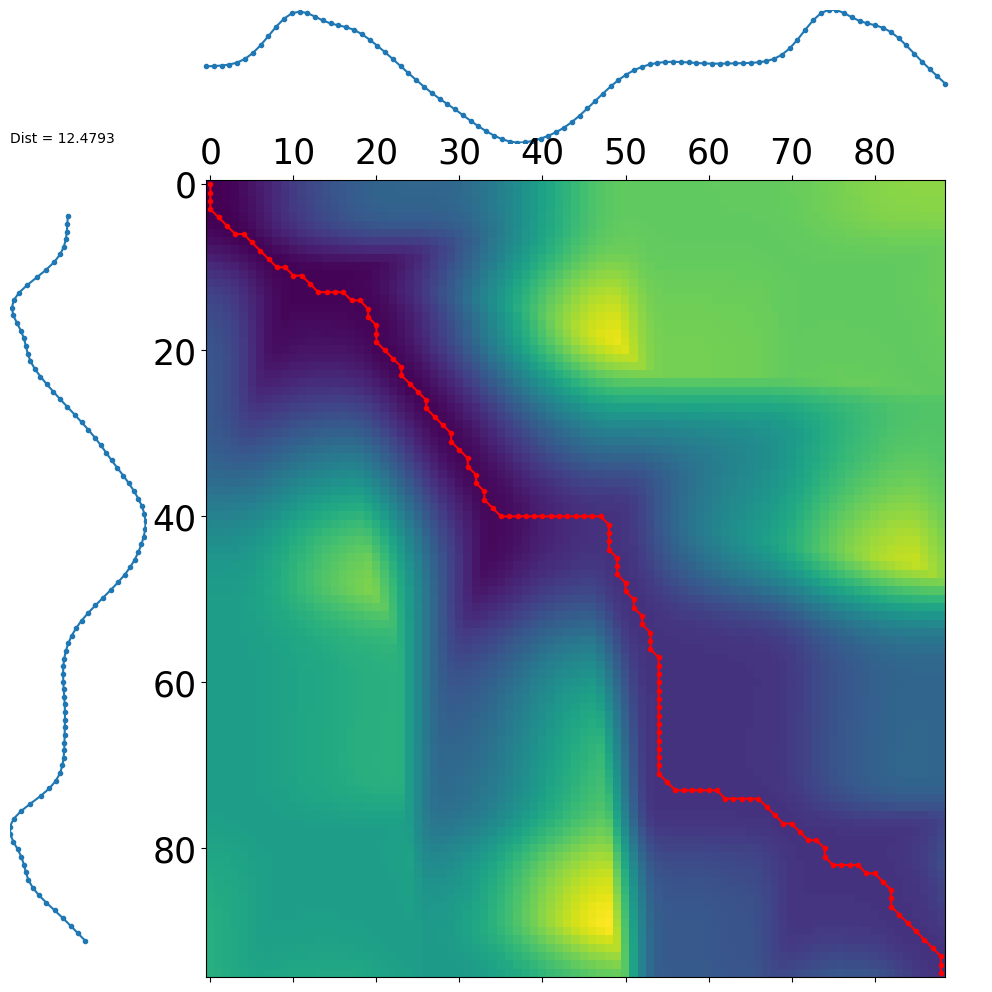
\includegraphics[width=0.49\textwidth]{machine-learning/warping_path_2_curves.png}
    \caption{An illustration of \acrshort{dtw} distance. The big coloured square is the \acrshort{lcm}, each monochromatic subsquare in is an entry in the \acrshort{lcm}. The color of each subsquare indicates the magnitude of the quadratic distance in that entry, blue indicates low, and green and yellow indicate higher values. The red line is the warping path.}
    \label{fig:warping_path}
\end{figure}

\subsection{Agglomerative Hierarchical Clustering} \label{sec:ahc}

The agglomerative hierarchical clustering algorithm is the chosen clustering algorithm in this work. It is a \textit{hard} clustering algorithm, meaning that data objects are given a single cluster assignment, and do not have partial memberships to many different clusters. Clustering algorithms that assign data objects partial memberships to many clusters are called \textit{soft} clustering algorithms. \bigskip

\textit{Partitional clustering algorithms} is a family of clustering algorithms that is an alternative to the family of hierarchical clustering algorithms. Partitional methods work iteratively and rely on defining prototypes that represent the cluster center. In the first iteration, the prototypes are randomly initialized. Then, the dissimilarity between all data objects and the prototypes are calculated, the data objects are then assigned to the cluster where the dissimilarity to the cluster prototype is minimal. The final step is to update the cluster prototypes such that they best represent the center of the new cluster. These steps repeat until the value of the cluster prototypes, and cluster membership assignments converge. \bigskip

Hierarchical clustering algorithms have two central advantages over partitional clustering algorithms, such as K-means, K-medoids, and fuzzy C-means. The first advantage is that the user does not have to decide the number of clusters they want to partition the dataset into prior to using the algorithm. The second is that due to the reliance on cluster prototypes and their random initialization, the cluster assignments yielded when the partitional algorithm are non-deterministic. The clusters assignments that a partitional algorithm converges to is dependent on what values the cluster prototypes are given upon initialization. Hierarchical clustering algorithms will always yield the same hierarchy of cluster assignments, given that the same dissimilarity matrix is inputted. \bigskip

There are two main types of hierarchical clustering algorithms, \textit{divisive} and \textit{agglomerative}. To understand the difference between these two algorithms, it helps to first understand how agglomerative hierarchical clustering works. Assume one is applying the hierarchical clustering algorithm to cluster a dataset of $N$ data objects. In the initial step, the algorithm takes the dissimilarity matrix as input, and every data object in the dataset is regarded as a separate cluster. Next, the case of $N-1$ clusters is considered, two of the existing clusters are merged based on which clusters have the lowest dissimilarity such that there then are $N-1$ clusters. The dissimilarity between clusters is estimated with what is called a \textit{linkage criterion}, which will be expanded upon later. This step of merging existing clusters is repeated until all data objects are contained in one cluster. The result is a hierarchy of clusters called a \textit{dendrogram}, that can yield cluster assignments at all the possible number of clusters. If one says that agglomerative hierarchical clustering has a bottom-top approach, divisive hierarchical clustering can be said to have a top-bottom approach. It starts at the top of the dendrogram with all data objects in one cluster and continuously splits the cluster until every object is contained in its own cluster. In this work, seven different linkage criteria are used, as detailed below.

\begin{itemize}
    \item \textbf{Single linkage}: Computes the dissimilarity between two clusters as the smallest dissimilarity between two individual members of each cluster \cite{dependency_tsc_energy_markets}.
    \item \textbf{Complete linkage}: Computes the dissimilarity between two clusters as the biggest dissimilarity between two individual members of each cluster \cite{financial_tsc_variance_ratio}.
    \item \textbf{Average linkage}: Computes the dissimilarity between two clusters as the average dissimilarity between all members of each cluster \cite{dependency_tsc_energy_markets}.
    \item \textbf{Ward linkage}: Computes the dissimilarity between two clusters as the increase in sum squared dissimilarity of the entire cluster that would be the result of merging the two clusters \cite{copula_ica_tsc}.
    \item \textbf{Centroid linkage}: Computes the dissimilarity between clusters by representing each cluster with a ''centroid'', which is another word for a cluster prototype. The dissimilarity between clusters is then computed as the dissimilarity between the centroids of each cluster. After the two clusters are merged, a new centroid is computed based on all the cluster members of the two clusters merged \cite{scipy_hier_reference}.
    \item \textbf{Median linkage}: Computes dissimilarity between two clusters in the same way as the centroid linkage, the only difference being that after the clusters are merged, the new centroid is computed as the average of the two previous centroids \cite{scipy_hier_reference}.
    \item \textbf{Weighted linkage}: Works in a method similar to the average linkage, the only difference being that after two clusters are merged, this linkage requires all the entries in the dissimilarity matrix that pertain to members of this cluster to be averaged. This merging of entries in the dissimilarity matrix reduces the number of computations required further down the line because there will be fewer dissimilarity values to average \cite{scipy_hier_reference}.
\end{itemize}

One of the apparent disadvantages of the hierarchical clustering algorithms is that they have quadratic time complexity $O(N^2)$, and have also received critique for lacking flexibility \cite{tsc_rev}. The lack of flexibility is because after two clusters are merged, they cannot be split for re-evaluation when a lower number of clusters is considered. 

\subsection{Curse of Dimensionality} \label{sec:curse_dimensionality}
The curse of dimensionality is a term used to explain the problem of having \textit{too much} information about each individual object, with regard to the number of objects that make up the dataset. This concept may sound counterintuitive, but it is a real issue in classification and regression problems. For every new parameter that is added to a data object (or every dimension that is added to a dataset), additional undesired stochastic behavior is added as well. Undesired stochastic behavior is often referred to as \textit{noise} because it makes it harder to detect the relation between the input variables and the target variable. If the amount of noise in a dataset becomes high enough, a machine learning model will become unable to generalize the relationship between the input variables and the target variables. The curse of dimensionality refers to the issue of the noise that is added when too many dimensions have been used to represent a dataset. The number of dimensions must be chosen in the context of how many objects there are in the dataset because if the number of objects in the dataset is great enough, the information added by an additional dimension could outweigh the additional noise cost.

\clearpage

\section{Artificial Neural Networks} \label{sec:ann}

This section will explain how layers of perceptrons form an \acrfull{ann}, how the said network is trained, the function of convolutional and recurrent layers in an \acrshort{ann}, and will discuss the challenges of underfitting and overfitting.

\subsection{Multi-layer Perceptrons} \label{sec:mlp}
Figure \ref{fig:perc_nn}a depicts the building blocks of an \acrshort{ann}, the perceptron. 
The perceptron is a model of an artificial neuron, it takes in $n$ inputs, performs a weighted sum of the inputs and a bias $b$, and sends the sum through what is called an activation function. A single perceptron is only able to perform binary classification on linearly separable points. However, by combining multiple perceptrons into a layer, and multiple layers of perceptrons into a \acrfull{mlp}, they can capture complex non-linear relationships. 

\begin{figure}[H]
\begin{center}
    \tikzstyle{init} = [pin edge={to-,thin,black}]
\tikzstyle{circ} = [circle, minimum size=1cm, text centered, draw=black, fill=blue!20]
\tikzstyle{arrow} = [thin,->,>=stealth]
\tikzstyle{arrow_t} = [very thin,->,>=stealth]

\tikzstyle{perc_in} = [circle, minimum size=1mm, text centered, draw=black, fill=blue!20]
\tikzstyle{perc_ou} = [circle, minimum size=1mm, text centered, draw=black, fill=red!20]
\tikzstyle{perc_hi} = [circle, minimum size=1mm, text centered, draw=black, fill=green!20]

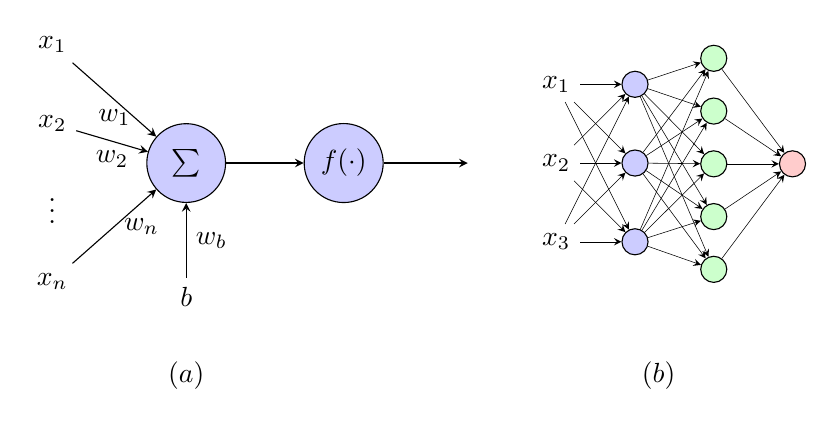
\begin{tikzpicture}
% Perceptron
\node (x1) [init] {$x_1$};
\node (x2) [init, below of=x1] {$x_2$};
\node (vdots) [init, below of=x2] {$\vdots$};
\node (xn) [init, below of=vdots] {$x_n$};

\node (sum) [circ, right of=x2, xshift=0.7cm, yshift=-5mm] {$\sum$};
\node (b) [init, below of=sum, yshift=-0.7cm] {$b$};
\node (obj) [circ, right of=sum, xshift=1cm] {$f(\cdot)$};
\node (output) [init, right of=obj, xshift=0.7cm] {};

\draw [arrow] (x1) --node[anchor=north] {$w_1$} (sum);
\draw [arrow] (x2) --node[anchor=north] {$w_2$} (sum);
\draw [arrow] (xn) --node[anchor=west] {$w_n$} (sum);
\draw [arrow] (b) --node[anchor=west] {$w_b$} (sum);
\draw [arrow] (sum) -- (obj);
\draw [arrow] (obj) -- (output);

% ANN
\node (i2) [init, right of=output] {$x_2$};
\node (i1) [init,, above of=i2] {$x_1$};
\node (i3) [init, below of=i2] {$x_3$};

\node (in0) [perc_in, right of=i1] {};
\node (in1) [perc_in, below of=in0] {};
\node (in2) [perc_in, below of=in1] {};

\node (hi0) [perc_hi, right of=in0, yshift=3.3mm] {};
\node (hi1) [perc_hi, below of=hi0, yshift=3.3mm] {};
\node (hi2) [perc_hi, below of=hi1, yshift=3.3mm] {};
\node (hi3) [perc_hi, below of=hi2, yshift=3.3mm] {};
\node (hi4) [perc_hi, below of=hi3, yshift=3.3mm] {};

\node (ou0) [perc_ou, right of=hi2] {};

\draw [arrow_t] (i1) -- (in0);
\draw [arrow_t] (i1) -- (in1);
\draw [arrow_t] (i1) -- (in2);
\draw [arrow_t] (i2) -- (in0);
\draw [arrow_t] (i2) -- (in1);
\draw [arrow_t] (i2) -- (in2);
\draw [arrow_t] (i3) -- (in0);
\draw [arrow_t] (i3) -- (in1);
\draw [arrow_t] (i3) -- (in2);

\draw [arrow_t] (in0) -- (hi0);
\draw [arrow_t] (in0) -- (hi1);
\draw [arrow_t] (in0) -- (hi2);
\draw [arrow_t] (in0) -- (hi3);
\draw [arrow_t] (in0) -- (hi4);
\draw [arrow_t] (in1) -- (hi0);
\draw [arrow_t] (in1) -- (hi1);
\draw [arrow_t] (in1) -- (hi2);
\draw [arrow_t] (in1) -- (hi3);
\draw [arrow_t] (in1) -- (hi4);
\draw [arrow_t] (in2) -- (hi0);
\draw [arrow_t] (in2) -- (hi1);
\draw [arrow_t] (in2) -- (hi2);
\draw [arrow_t] (in2) -- (hi3);
\draw [arrow_t] (in2) -- (hi4);

\draw [arrow_t] (hi0) -- (ou0);
\draw [arrow_t] (hi1) -- (ou0);
\draw [arrow_t] (hi2) -- (ou0);
\draw [arrow_t] (hi3) -- (ou0);
\draw [arrow_t] (hi4) -- (ou0);

\node (label_a) [init, below of=b] {$(a)$};
\node (label_a) [init, right of=label_a, xshift=5cm] {$(b)$};
\end{tikzpicture}
\end{center}
\caption{$(a)$ A Perceptron. $(b)$ Example of a simple \acrshort{ann} known as an \acrshort{mlp}.} 
\label{fig:perc_nn}
\end{figure}

\begin{equation}
    O(\mathbf{x}) = f \left ( \sum_{i = 1}^N w_i x_i + w_b b\right )
    \label{eq:perc}
\end{equation}

Equation \eqref{eq:perc} shows what the output of a perceptron ($O(\mathbf{x})$) is in terms of its weights $\{w_i\}$, the input $\mathbf{x}$, its activation function $f(\cdot)$ and its bias $b$. The purpose of an activation function is to give each perceptron the ability to perform actions that are not purely linear on its inputs \cite{dl_book}. Consider that the absence of an activation function, all a perceptron is doing is outputting a weighted sum of its inputs. Any continuous function can, in principle, be used as an activation function, but some functions are more common than others. Figure \ref{fig:obj_funcs} shows the three most popular activation functions used in modern \acrshort{ann}, the sigmoid function, $\mathrm{tanh}$ function, and \acrfull{relu}. The sigmoid function was one of the first activation functions introduced, and it shares many similar characteristics with the $\mathrm{tanh}$ function. The sigmoid, and $\mathrm{tanh}$ functions are both hyperbolic functions that grant non-linear properties to the perceptron. However, the \acrshort{relu} function is often preferred over the two former functions for two important reasons. First, the hyperbolic functions suffer an issue of saturation when the weighted sums of the input becomes sufficiently large, while the \acrshort{relu} does not. The second reason is not as technical, but is still important. Since an \acrshort{ann} can be made up of hundreds, or even thousands of perceptrons, the computation of complex exponential functions for every unit is computationally expensive, whereas the computation of the \acrshort{relu} is significantly less so. 

\begin{figure}[H]
    \centering
    \begin{subfigure}[b]{0.32\textwidth}
        \centering
        %% Creator: Matplotlib, PGF backend
%%
%% To include the figure in your LaTeX document, write
%%   \input{<filename>.pgf}
%%
%% Make sure the required packages are loaded in your preamble
%%   \usepackage{pgf}
%%
%% Figures using additional raster images can only be included by \input if
%% they are in the same directory as the main LaTeX file. For loading figures
%% from other directories you can use the `import` package
%%   \usepackage{import}
%% and then include the figures with
%%   \import{<path to file>}{<filename>.pgf}
%%
%% Matplotlib used the following preamble
%%
\begingroup%
\makeatletter%
\begin{pgfpicture}%
\pgfpathrectangle{\pgfpointorigin}{\pgfqpoint{1.900000in}{1.900000in}}%
\pgfusepath{use as bounding box, clip}%
\begin{pgfscope}%
\pgfsetbuttcap%
\pgfsetmiterjoin%
\definecolor{currentfill}{rgb}{1.000000,1.000000,1.000000}%
\pgfsetfillcolor{currentfill}%
\pgfsetlinewidth{0.000000pt}%
\definecolor{currentstroke}{rgb}{1.000000,1.000000,1.000000}%
\pgfsetstrokecolor{currentstroke}%
\pgfsetdash{}{0pt}%
\pgfpathmoveto{\pgfqpoint{0.000000in}{0.000000in}}%
\pgfpathlineto{\pgfqpoint{1.900000in}{0.000000in}}%
\pgfpathlineto{\pgfqpoint{1.900000in}{1.900000in}}%
\pgfpathlineto{\pgfqpoint{0.000000in}{1.900000in}}%
\pgfpathclose%
\pgfusepath{fill}%
\end{pgfscope}%
\begin{pgfscope}%
\pgfsetbuttcap%
\pgfsetmiterjoin%
\definecolor{currentfill}{rgb}{1.000000,1.000000,1.000000}%
\pgfsetfillcolor{currentfill}%
\pgfsetlinewidth{0.000000pt}%
\definecolor{currentstroke}{rgb}{0.000000,0.000000,0.000000}%
\pgfsetstrokecolor{currentstroke}%
\pgfsetstrokeopacity{0.000000}%
\pgfsetdash{}{0pt}%
\pgfpathmoveto{\pgfqpoint{0.461302in}{0.308333in}}%
\pgfpathlineto{\pgfqpoint{1.800000in}{0.308333in}}%
\pgfpathlineto{\pgfqpoint{1.800000in}{1.800000in}}%
\pgfpathlineto{\pgfqpoint{0.461302in}{1.800000in}}%
\pgfpathclose%
\pgfusepath{fill}%
\end{pgfscope}%
\begin{pgfscope}%
\pgfsetbuttcap%
\pgfsetroundjoin%
\definecolor{currentfill}{rgb}{0.000000,0.000000,0.000000}%
\pgfsetfillcolor{currentfill}%
\pgfsetlinewidth{0.803000pt}%
\definecolor{currentstroke}{rgb}{0.000000,0.000000,0.000000}%
\pgfsetstrokecolor{currentstroke}%
\pgfsetdash{}{0pt}%
\pgfsys@defobject{currentmarker}{\pgfqpoint{0.000000in}{-0.048611in}}{\pgfqpoint{0.000000in}{0.000000in}}{%
\pgfpathmoveto{\pgfqpoint{0.000000in}{0.000000in}}%
\pgfpathlineto{\pgfqpoint{0.000000in}{-0.048611in}}%
\pgfusepath{stroke,fill}%
}%
\begin{pgfscope}%
\pgfsys@transformshift{0.522152in}{0.308333in}%
\pgfsys@useobject{currentmarker}{}%
\end{pgfscope}%
\end{pgfscope}%
\begin{pgfscope}%
\definecolor{textcolor}{rgb}{0.000000,0.000000,0.000000}%
\pgfsetstrokecolor{textcolor}%
\pgfsetfillcolor{textcolor}%
\pgftext[x=0.522152in,y=0.211111in,,top]{\color{textcolor}\rmfamily\fontsize{9.000000}{10.800000}\selectfont \(\displaystyle -5\)}%
\end{pgfscope}%
\begin{pgfscope}%
\pgfsetbuttcap%
\pgfsetroundjoin%
\definecolor{currentfill}{rgb}{0.000000,0.000000,0.000000}%
\pgfsetfillcolor{currentfill}%
\pgfsetlinewidth{0.803000pt}%
\definecolor{currentstroke}{rgb}{0.000000,0.000000,0.000000}%
\pgfsetstrokecolor{currentstroke}%
\pgfsetdash{}{0pt}%
\pgfsys@defobject{currentmarker}{\pgfqpoint{0.000000in}{-0.048611in}}{\pgfqpoint{0.000000in}{0.000000in}}{%
\pgfpathmoveto{\pgfqpoint{0.000000in}{0.000000in}}%
\pgfpathlineto{\pgfqpoint{0.000000in}{-0.048611in}}%
\pgfusepath{stroke,fill}%
}%
\begin{pgfscope}%
\pgfsys@transformshift{1.130651in}{0.308333in}%
\pgfsys@useobject{currentmarker}{}%
\end{pgfscope}%
\end{pgfscope}%
\begin{pgfscope}%
\definecolor{textcolor}{rgb}{0.000000,0.000000,0.000000}%
\pgfsetstrokecolor{textcolor}%
\pgfsetfillcolor{textcolor}%
\pgftext[x=1.130651in,y=0.211111in,,top]{\color{textcolor}\rmfamily\fontsize{9.000000}{10.800000}\selectfont \(\displaystyle 0\)}%
\end{pgfscope}%
\begin{pgfscope}%
\pgfsetbuttcap%
\pgfsetroundjoin%
\definecolor{currentfill}{rgb}{0.000000,0.000000,0.000000}%
\pgfsetfillcolor{currentfill}%
\pgfsetlinewidth{0.803000pt}%
\definecolor{currentstroke}{rgb}{0.000000,0.000000,0.000000}%
\pgfsetstrokecolor{currentstroke}%
\pgfsetdash{}{0pt}%
\pgfsys@defobject{currentmarker}{\pgfqpoint{0.000000in}{-0.048611in}}{\pgfqpoint{0.000000in}{0.000000in}}{%
\pgfpathmoveto{\pgfqpoint{0.000000in}{0.000000in}}%
\pgfpathlineto{\pgfqpoint{0.000000in}{-0.048611in}}%
\pgfusepath{stroke,fill}%
}%
\begin{pgfscope}%
\pgfsys@transformshift{1.739150in}{0.308333in}%
\pgfsys@useobject{currentmarker}{}%
\end{pgfscope}%
\end{pgfscope}%
\begin{pgfscope}%
\definecolor{textcolor}{rgb}{0.000000,0.000000,0.000000}%
\pgfsetstrokecolor{textcolor}%
\pgfsetfillcolor{textcolor}%
\pgftext[x=1.739150in,y=0.211111in,,top]{\color{textcolor}\rmfamily\fontsize{9.000000}{10.800000}\selectfont \(\displaystyle 5\)}%
\end{pgfscope}%
\begin{pgfscope}%
\pgfsetbuttcap%
\pgfsetroundjoin%
\definecolor{currentfill}{rgb}{0.000000,0.000000,0.000000}%
\pgfsetfillcolor{currentfill}%
\pgfsetlinewidth{0.803000pt}%
\definecolor{currentstroke}{rgb}{0.000000,0.000000,0.000000}%
\pgfsetstrokecolor{currentstroke}%
\pgfsetdash{}{0pt}%
\pgfsys@defobject{currentmarker}{\pgfqpoint{-0.048611in}{0.000000in}}{\pgfqpoint{0.000000in}{0.000000in}}{%
\pgfpathmoveto{\pgfqpoint{0.000000in}{0.000000in}}%
\pgfpathlineto{\pgfqpoint{-0.048611in}{0.000000in}}%
\pgfusepath{stroke,fill}%
}%
\begin{pgfscope}%
\pgfsys@transformshift{0.461302in}{0.376136in}%
\pgfsys@useobject{currentmarker}{}%
\end{pgfscope}%
\end{pgfscope}%
\begin{pgfscope}%
\definecolor{textcolor}{rgb}{0.000000,0.000000,0.000000}%
\pgfsetstrokecolor{textcolor}%
\pgfsetfillcolor{textcolor}%
\pgftext[x=0.100000in,y=0.332734in,left,base]{\color{textcolor}\rmfamily\fontsize{9.000000}{10.800000}\selectfont \(\displaystyle -1.0\)}%
\end{pgfscope}%
\begin{pgfscope}%
\pgfsetbuttcap%
\pgfsetroundjoin%
\definecolor{currentfill}{rgb}{0.000000,0.000000,0.000000}%
\pgfsetfillcolor{currentfill}%
\pgfsetlinewidth{0.803000pt}%
\definecolor{currentstroke}{rgb}{0.000000,0.000000,0.000000}%
\pgfsetstrokecolor{currentstroke}%
\pgfsetdash{}{0pt}%
\pgfsys@defobject{currentmarker}{\pgfqpoint{-0.048611in}{0.000000in}}{\pgfqpoint{0.000000in}{0.000000in}}{%
\pgfpathmoveto{\pgfqpoint{0.000000in}{0.000000in}}%
\pgfpathlineto{\pgfqpoint{-0.048611in}{0.000000in}}%
\pgfusepath{stroke,fill}%
}%
\begin{pgfscope}%
\pgfsys@transformshift{0.461302in}{0.715152in}%
\pgfsys@useobject{currentmarker}{}%
\end{pgfscope}%
\end{pgfscope}%
\begin{pgfscope}%
\definecolor{textcolor}{rgb}{0.000000,0.000000,0.000000}%
\pgfsetstrokecolor{textcolor}%
\pgfsetfillcolor{textcolor}%
\pgftext[x=0.100000in,y=0.671749in,left,base]{\color{textcolor}\rmfamily\fontsize{9.000000}{10.800000}\selectfont \(\displaystyle -0.5\)}%
\end{pgfscope}%
\begin{pgfscope}%
\pgfsetbuttcap%
\pgfsetroundjoin%
\definecolor{currentfill}{rgb}{0.000000,0.000000,0.000000}%
\pgfsetfillcolor{currentfill}%
\pgfsetlinewidth{0.803000pt}%
\definecolor{currentstroke}{rgb}{0.000000,0.000000,0.000000}%
\pgfsetstrokecolor{currentstroke}%
\pgfsetdash{}{0pt}%
\pgfsys@defobject{currentmarker}{\pgfqpoint{-0.048611in}{0.000000in}}{\pgfqpoint{0.000000in}{0.000000in}}{%
\pgfpathmoveto{\pgfqpoint{0.000000in}{0.000000in}}%
\pgfpathlineto{\pgfqpoint{-0.048611in}{0.000000in}}%
\pgfusepath{stroke,fill}%
}%
\begin{pgfscope}%
\pgfsys@transformshift{0.461302in}{1.054167in}%
\pgfsys@useobject{currentmarker}{}%
\end{pgfscope}%
\end{pgfscope}%
\begin{pgfscope}%
\definecolor{textcolor}{rgb}{0.000000,0.000000,0.000000}%
\pgfsetstrokecolor{textcolor}%
\pgfsetfillcolor{textcolor}%
\pgftext[x=0.199922in,y=1.010764in,left,base]{\color{textcolor}\rmfamily\fontsize{9.000000}{10.800000}\selectfont \(\displaystyle 0.0\)}%
\end{pgfscope}%
\begin{pgfscope}%
\pgfsetbuttcap%
\pgfsetroundjoin%
\definecolor{currentfill}{rgb}{0.000000,0.000000,0.000000}%
\pgfsetfillcolor{currentfill}%
\pgfsetlinewidth{0.803000pt}%
\definecolor{currentstroke}{rgb}{0.000000,0.000000,0.000000}%
\pgfsetstrokecolor{currentstroke}%
\pgfsetdash{}{0pt}%
\pgfsys@defobject{currentmarker}{\pgfqpoint{-0.048611in}{0.000000in}}{\pgfqpoint{0.000000in}{0.000000in}}{%
\pgfpathmoveto{\pgfqpoint{0.000000in}{0.000000in}}%
\pgfpathlineto{\pgfqpoint{-0.048611in}{0.000000in}}%
\pgfusepath{stroke,fill}%
}%
\begin{pgfscope}%
\pgfsys@transformshift{0.461302in}{1.393182in}%
\pgfsys@useobject{currentmarker}{}%
\end{pgfscope}%
\end{pgfscope}%
\begin{pgfscope}%
\definecolor{textcolor}{rgb}{0.000000,0.000000,0.000000}%
\pgfsetstrokecolor{textcolor}%
\pgfsetfillcolor{textcolor}%
\pgftext[x=0.199922in,y=1.349779in,left,base]{\color{textcolor}\rmfamily\fontsize{9.000000}{10.800000}\selectfont \(\displaystyle 0.5\)}%
\end{pgfscope}%
\begin{pgfscope}%
\pgfsetbuttcap%
\pgfsetroundjoin%
\definecolor{currentfill}{rgb}{0.000000,0.000000,0.000000}%
\pgfsetfillcolor{currentfill}%
\pgfsetlinewidth{0.803000pt}%
\definecolor{currentstroke}{rgb}{0.000000,0.000000,0.000000}%
\pgfsetstrokecolor{currentstroke}%
\pgfsetdash{}{0pt}%
\pgfsys@defobject{currentmarker}{\pgfqpoint{-0.048611in}{0.000000in}}{\pgfqpoint{0.000000in}{0.000000in}}{%
\pgfpathmoveto{\pgfqpoint{0.000000in}{0.000000in}}%
\pgfpathlineto{\pgfqpoint{-0.048611in}{0.000000in}}%
\pgfusepath{stroke,fill}%
}%
\begin{pgfscope}%
\pgfsys@transformshift{0.461302in}{1.732197in}%
\pgfsys@useobject{currentmarker}{}%
\end{pgfscope}%
\end{pgfscope}%
\begin{pgfscope}%
\definecolor{textcolor}{rgb}{0.000000,0.000000,0.000000}%
\pgfsetstrokecolor{textcolor}%
\pgfsetfillcolor{textcolor}%
\pgftext[x=0.199922in,y=1.688794in,left,base]{\color{textcolor}\rmfamily\fontsize{9.000000}{10.800000}\selectfont \(\displaystyle 1.0\)}%
\end{pgfscope}%
\begin{pgfscope}%
\pgfpathrectangle{\pgfqpoint{0.461302in}{0.308333in}}{\pgfqpoint{1.338698in}{1.491667in}}%
\pgfusepath{clip}%
\pgfsetrectcap%
\pgfsetroundjoin%
\pgfsetlinewidth{1.505625pt}%
\definecolor{currentstroke}{rgb}{0.121569,0.466667,0.705882}%
\pgfsetstrokecolor{currentstroke}%
\pgfsetdash{}{0pt}%
\pgfpathmoveto{\pgfqpoint{0.522152in}{1.058705in}}%
\pgfpathlineto{\pgfqpoint{0.601655in}{1.062834in}}%
\pgfpathlineto{\pgfqpoint{0.656695in}{1.067692in}}%
\pgfpathlineto{\pgfqpoint{0.705619in}{1.074187in}}%
\pgfpathlineto{\pgfqpoint{0.748428in}{1.082277in}}%
\pgfpathlineto{\pgfqpoint{0.785122in}{1.091623in}}%
\pgfpathlineto{\pgfqpoint{0.815699in}{1.101574in}}%
\pgfpathlineto{\pgfqpoint{0.846277in}{1.113922in}}%
\pgfpathlineto{\pgfqpoint{0.876855in}{1.129103in}}%
\pgfpathlineto{\pgfqpoint{0.901317in}{1.143587in}}%
\pgfpathlineto{\pgfqpoint{0.925780in}{1.160376in}}%
\pgfpathlineto{\pgfqpoint{0.950242in}{1.179645in}}%
\pgfpathlineto{\pgfqpoint{0.974704in}{1.201510in}}%
\pgfpathlineto{\pgfqpoint{0.999166in}{1.226000in}}%
\pgfpathlineto{\pgfqpoint{1.029744in}{1.260170in}}%
\pgfpathlineto{\pgfqpoint{1.060322in}{1.297863in}}%
\pgfpathlineto{\pgfqpoint{1.097015in}{1.346629in}}%
\pgfpathlineto{\pgfqpoint{1.207096in}{1.496288in}}%
\pgfpathlineto{\pgfqpoint{1.237674in}{1.533329in}}%
\pgfpathlineto{\pgfqpoint{1.268251in}{1.566730in}}%
\pgfpathlineto{\pgfqpoint{1.292714in}{1.590566in}}%
\pgfpathlineto{\pgfqpoint{1.317176in}{1.611776in}}%
\pgfpathlineto{\pgfqpoint{1.341638in}{1.630412in}}%
\pgfpathlineto{\pgfqpoint{1.366100in}{1.646606in}}%
\pgfpathlineto{\pgfqpoint{1.390563in}{1.660545in}}%
\pgfpathlineto{\pgfqpoint{1.421141in}{1.675124in}}%
\pgfpathlineto{\pgfqpoint{1.451718in}{1.686958in}}%
\pgfpathlineto{\pgfqpoint{1.482296in}{1.696480in}}%
\pgfpathlineto{\pgfqpoint{1.518990in}{1.705410in}}%
\pgfpathlineto{\pgfqpoint{1.561799in}{1.713130in}}%
\pgfpathlineto{\pgfqpoint{1.610723in}{1.719322in}}%
\pgfpathlineto{\pgfqpoint{1.665763in}{1.723949in}}%
\pgfpathlineto{\pgfqpoint{1.739150in}{1.727659in}}%
\pgfpathlineto{\pgfqpoint{1.739150in}{1.727659in}}%
\pgfusepath{stroke}%
\end{pgfscope}%
\begin{pgfscope}%
\pgfsetrectcap%
\pgfsetmiterjoin%
\pgfsetlinewidth{0.803000pt}%
\definecolor{currentstroke}{rgb}{0.000000,0.000000,0.000000}%
\pgfsetstrokecolor{currentstroke}%
\pgfsetdash{}{0pt}%
\pgfpathmoveto{\pgfqpoint{0.461302in}{0.308333in}}%
\pgfpathlineto{\pgfqpoint{0.461302in}{1.800000in}}%
\pgfusepath{stroke}%
\end{pgfscope}%
\begin{pgfscope}%
\pgfsetrectcap%
\pgfsetmiterjoin%
\pgfsetlinewidth{0.803000pt}%
\definecolor{currentstroke}{rgb}{0.000000,0.000000,0.000000}%
\pgfsetstrokecolor{currentstroke}%
\pgfsetdash{}{0pt}%
\pgfpathmoveto{\pgfqpoint{1.800000in}{0.308333in}}%
\pgfpathlineto{\pgfqpoint{1.800000in}{1.800000in}}%
\pgfusepath{stroke}%
\end{pgfscope}%
\begin{pgfscope}%
\pgfsetrectcap%
\pgfsetmiterjoin%
\pgfsetlinewidth{0.803000pt}%
\definecolor{currentstroke}{rgb}{0.000000,0.000000,0.000000}%
\pgfsetstrokecolor{currentstroke}%
\pgfsetdash{}{0pt}%
\pgfpathmoveto{\pgfqpoint{0.461302in}{0.308333in}}%
\pgfpathlineto{\pgfqpoint{1.800000in}{0.308333in}}%
\pgfusepath{stroke}%
\end{pgfscope}%
\begin{pgfscope}%
\pgfsetrectcap%
\pgfsetmiterjoin%
\pgfsetlinewidth{0.803000pt}%
\definecolor{currentstroke}{rgb}{0.000000,0.000000,0.000000}%
\pgfsetstrokecolor{currentstroke}%
\pgfsetdash{}{0pt}%
\pgfpathmoveto{\pgfqpoint{0.461302in}{1.800000in}}%
\pgfpathlineto{\pgfqpoint{1.800000in}{1.800000in}}%
\pgfusepath{stroke}%
\end{pgfscope}%
\end{pgfpicture}%
\makeatother%
\endgroup%

        \caption{$\mathrm{sigmoid}(x) = \frac{1}{1+e^{-x}}$}
        \label{fig:sigmoid}
    \end{subfigure}
    \begin{subfigure}[b]{0.32\textwidth}
        \centering
        %% Creator: Matplotlib, PGF backend
%%
%% To include the figure in your LaTeX document, write
%%   \input{<filename>.pgf}
%%
%% Make sure the required packages are loaded in your preamble
%%   \usepackage{pgf}
%%
%% Figures using additional raster images can only be included by \input if
%% they are in the same directory as the main LaTeX file. For loading figures
%% from other directories you can use the `import` package
%%   \usepackage{import}
%% and then include the figures with
%%   \import{<path to file>}{<filename>.pgf}
%%
%% Matplotlib used the following preamble
%%
\begingroup%
\makeatletter%
\begin{pgfpicture}%
\pgfpathrectangle{\pgfpointorigin}{\pgfqpoint{1.900000in}{1.900000in}}%
\pgfusepath{use as bounding box, clip}%
\begin{pgfscope}%
\pgfsetbuttcap%
\pgfsetmiterjoin%
\definecolor{currentfill}{rgb}{1.000000,1.000000,1.000000}%
\pgfsetfillcolor{currentfill}%
\pgfsetlinewidth{0.000000pt}%
\definecolor{currentstroke}{rgb}{1.000000,1.000000,1.000000}%
\pgfsetstrokecolor{currentstroke}%
\pgfsetdash{}{0pt}%
\pgfpathmoveto{\pgfqpoint{0.000000in}{0.000000in}}%
\pgfpathlineto{\pgfqpoint{1.900000in}{0.000000in}}%
\pgfpathlineto{\pgfqpoint{1.900000in}{1.900000in}}%
\pgfpathlineto{\pgfqpoint{0.000000in}{1.900000in}}%
\pgfpathclose%
\pgfusepath{fill}%
\end{pgfscope}%
\begin{pgfscope}%
\pgfsetbuttcap%
\pgfsetmiterjoin%
\definecolor{currentfill}{rgb}{1.000000,1.000000,1.000000}%
\pgfsetfillcolor{currentfill}%
\pgfsetlinewidth{0.000000pt}%
\definecolor{currentstroke}{rgb}{0.000000,0.000000,0.000000}%
\pgfsetstrokecolor{currentstroke}%
\pgfsetstrokeopacity{0.000000}%
\pgfsetdash{}{0pt}%
\pgfpathmoveto{\pgfqpoint{0.461302in}{0.308333in}}%
\pgfpathlineto{\pgfqpoint{1.800000in}{0.308333in}}%
\pgfpathlineto{\pgfqpoint{1.800000in}{1.800000in}}%
\pgfpathlineto{\pgfqpoint{0.461302in}{1.800000in}}%
\pgfpathclose%
\pgfusepath{fill}%
\end{pgfscope}%
\begin{pgfscope}%
\pgfsetbuttcap%
\pgfsetroundjoin%
\definecolor{currentfill}{rgb}{0.000000,0.000000,0.000000}%
\pgfsetfillcolor{currentfill}%
\pgfsetlinewidth{0.803000pt}%
\definecolor{currentstroke}{rgb}{0.000000,0.000000,0.000000}%
\pgfsetstrokecolor{currentstroke}%
\pgfsetdash{}{0pt}%
\pgfsys@defobject{currentmarker}{\pgfqpoint{0.000000in}{-0.048611in}}{\pgfqpoint{0.000000in}{0.000000in}}{%
\pgfpathmoveto{\pgfqpoint{0.000000in}{0.000000in}}%
\pgfpathlineto{\pgfqpoint{0.000000in}{-0.048611in}}%
\pgfusepath{stroke,fill}%
}%
\begin{pgfscope}%
\pgfsys@transformshift{0.522152in}{0.308333in}%
\pgfsys@useobject{currentmarker}{}%
\end{pgfscope}%
\end{pgfscope}%
\begin{pgfscope}%
\definecolor{textcolor}{rgb}{0.000000,0.000000,0.000000}%
\pgfsetstrokecolor{textcolor}%
\pgfsetfillcolor{textcolor}%
\pgftext[x=0.522152in,y=0.211111in,,top]{\color{textcolor}\rmfamily\fontsize{9.000000}{10.800000}\selectfont \(\displaystyle -5\)}%
\end{pgfscope}%
\begin{pgfscope}%
\pgfsetbuttcap%
\pgfsetroundjoin%
\definecolor{currentfill}{rgb}{0.000000,0.000000,0.000000}%
\pgfsetfillcolor{currentfill}%
\pgfsetlinewidth{0.803000pt}%
\definecolor{currentstroke}{rgb}{0.000000,0.000000,0.000000}%
\pgfsetstrokecolor{currentstroke}%
\pgfsetdash{}{0pt}%
\pgfsys@defobject{currentmarker}{\pgfqpoint{0.000000in}{-0.048611in}}{\pgfqpoint{0.000000in}{0.000000in}}{%
\pgfpathmoveto{\pgfqpoint{0.000000in}{0.000000in}}%
\pgfpathlineto{\pgfqpoint{0.000000in}{-0.048611in}}%
\pgfusepath{stroke,fill}%
}%
\begin{pgfscope}%
\pgfsys@transformshift{1.130651in}{0.308333in}%
\pgfsys@useobject{currentmarker}{}%
\end{pgfscope}%
\end{pgfscope}%
\begin{pgfscope}%
\definecolor{textcolor}{rgb}{0.000000,0.000000,0.000000}%
\pgfsetstrokecolor{textcolor}%
\pgfsetfillcolor{textcolor}%
\pgftext[x=1.130651in,y=0.211111in,,top]{\color{textcolor}\rmfamily\fontsize{9.000000}{10.800000}\selectfont \(\displaystyle 0\)}%
\end{pgfscope}%
\begin{pgfscope}%
\pgfsetbuttcap%
\pgfsetroundjoin%
\definecolor{currentfill}{rgb}{0.000000,0.000000,0.000000}%
\pgfsetfillcolor{currentfill}%
\pgfsetlinewidth{0.803000pt}%
\definecolor{currentstroke}{rgb}{0.000000,0.000000,0.000000}%
\pgfsetstrokecolor{currentstroke}%
\pgfsetdash{}{0pt}%
\pgfsys@defobject{currentmarker}{\pgfqpoint{0.000000in}{-0.048611in}}{\pgfqpoint{0.000000in}{0.000000in}}{%
\pgfpathmoveto{\pgfqpoint{0.000000in}{0.000000in}}%
\pgfpathlineto{\pgfqpoint{0.000000in}{-0.048611in}}%
\pgfusepath{stroke,fill}%
}%
\begin{pgfscope}%
\pgfsys@transformshift{1.739150in}{0.308333in}%
\pgfsys@useobject{currentmarker}{}%
\end{pgfscope}%
\end{pgfscope}%
\begin{pgfscope}%
\definecolor{textcolor}{rgb}{0.000000,0.000000,0.000000}%
\pgfsetstrokecolor{textcolor}%
\pgfsetfillcolor{textcolor}%
\pgftext[x=1.739150in,y=0.211111in,,top]{\color{textcolor}\rmfamily\fontsize{9.000000}{10.800000}\selectfont \(\displaystyle 5\)}%
\end{pgfscope}%
\begin{pgfscope}%
\pgfsetbuttcap%
\pgfsetroundjoin%
\definecolor{currentfill}{rgb}{0.000000,0.000000,0.000000}%
\pgfsetfillcolor{currentfill}%
\pgfsetlinewidth{0.803000pt}%
\definecolor{currentstroke}{rgb}{0.000000,0.000000,0.000000}%
\pgfsetstrokecolor{currentstroke}%
\pgfsetdash{}{0pt}%
\pgfsys@defobject{currentmarker}{\pgfqpoint{-0.048611in}{0.000000in}}{\pgfqpoint{0.000000in}{0.000000in}}{%
\pgfpathmoveto{\pgfqpoint{0.000000in}{0.000000in}}%
\pgfpathlineto{\pgfqpoint{-0.048611in}{0.000000in}}%
\pgfusepath{stroke,fill}%
}%
\begin{pgfscope}%
\pgfsys@transformshift{0.461302in}{0.376136in}%
\pgfsys@useobject{currentmarker}{}%
\end{pgfscope}%
\end{pgfscope}%
\begin{pgfscope}%
\definecolor{textcolor}{rgb}{0.000000,0.000000,0.000000}%
\pgfsetstrokecolor{textcolor}%
\pgfsetfillcolor{textcolor}%
\pgftext[x=0.100000in,y=0.332734in,left,base]{\color{textcolor}\rmfamily\fontsize{9.000000}{10.800000}\selectfont \(\displaystyle -1.0\)}%
\end{pgfscope}%
\begin{pgfscope}%
\pgfsetbuttcap%
\pgfsetroundjoin%
\definecolor{currentfill}{rgb}{0.000000,0.000000,0.000000}%
\pgfsetfillcolor{currentfill}%
\pgfsetlinewidth{0.803000pt}%
\definecolor{currentstroke}{rgb}{0.000000,0.000000,0.000000}%
\pgfsetstrokecolor{currentstroke}%
\pgfsetdash{}{0pt}%
\pgfsys@defobject{currentmarker}{\pgfqpoint{-0.048611in}{0.000000in}}{\pgfqpoint{0.000000in}{0.000000in}}{%
\pgfpathmoveto{\pgfqpoint{0.000000in}{0.000000in}}%
\pgfpathlineto{\pgfqpoint{-0.048611in}{0.000000in}}%
\pgfusepath{stroke,fill}%
}%
\begin{pgfscope}%
\pgfsys@transformshift{0.461302in}{0.715152in}%
\pgfsys@useobject{currentmarker}{}%
\end{pgfscope}%
\end{pgfscope}%
\begin{pgfscope}%
\definecolor{textcolor}{rgb}{0.000000,0.000000,0.000000}%
\pgfsetstrokecolor{textcolor}%
\pgfsetfillcolor{textcolor}%
\pgftext[x=0.100000in,y=0.671749in,left,base]{\color{textcolor}\rmfamily\fontsize{9.000000}{10.800000}\selectfont \(\displaystyle -0.5\)}%
\end{pgfscope}%
\begin{pgfscope}%
\pgfsetbuttcap%
\pgfsetroundjoin%
\definecolor{currentfill}{rgb}{0.000000,0.000000,0.000000}%
\pgfsetfillcolor{currentfill}%
\pgfsetlinewidth{0.803000pt}%
\definecolor{currentstroke}{rgb}{0.000000,0.000000,0.000000}%
\pgfsetstrokecolor{currentstroke}%
\pgfsetdash{}{0pt}%
\pgfsys@defobject{currentmarker}{\pgfqpoint{-0.048611in}{0.000000in}}{\pgfqpoint{0.000000in}{0.000000in}}{%
\pgfpathmoveto{\pgfqpoint{0.000000in}{0.000000in}}%
\pgfpathlineto{\pgfqpoint{-0.048611in}{0.000000in}}%
\pgfusepath{stroke,fill}%
}%
\begin{pgfscope}%
\pgfsys@transformshift{0.461302in}{1.054167in}%
\pgfsys@useobject{currentmarker}{}%
\end{pgfscope}%
\end{pgfscope}%
\begin{pgfscope}%
\definecolor{textcolor}{rgb}{0.000000,0.000000,0.000000}%
\pgfsetstrokecolor{textcolor}%
\pgfsetfillcolor{textcolor}%
\pgftext[x=0.199922in,y=1.010764in,left,base]{\color{textcolor}\rmfamily\fontsize{9.000000}{10.800000}\selectfont \(\displaystyle 0.0\)}%
\end{pgfscope}%
\begin{pgfscope}%
\pgfsetbuttcap%
\pgfsetroundjoin%
\definecolor{currentfill}{rgb}{0.000000,0.000000,0.000000}%
\pgfsetfillcolor{currentfill}%
\pgfsetlinewidth{0.803000pt}%
\definecolor{currentstroke}{rgb}{0.000000,0.000000,0.000000}%
\pgfsetstrokecolor{currentstroke}%
\pgfsetdash{}{0pt}%
\pgfsys@defobject{currentmarker}{\pgfqpoint{-0.048611in}{0.000000in}}{\pgfqpoint{0.000000in}{0.000000in}}{%
\pgfpathmoveto{\pgfqpoint{0.000000in}{0.000000in}}%
\pgfpathlineto{\pgfqpoint{-0.048611in}{0.000000in}}%
\pgfusepath{stroke,fill}%
}%
\begin{pgfscope}%
\pgfsys@transformshift{0.461302in}{1.393182in}%
\pgfsys@useobject{currentmarker}{}%
\end{pgfscope}%
\end{pgfscope}%
\begin{pgfscope}%
\definecolor{textcolor}{rgb}{0.000000,0.000000,0.000000}%
\pgfsetstrokecolor{textcolor}%
\pgfsetfillcolor{textcolor}%
\pgftext[x=0.199922in,y=1.349779in,left,base]{\color{textcolor}\rmfamily\fontsize{9.000000}{10.800000}\selectfont \(\displaystyle 0.5\)}%
\end{pgfscope}%
\begin{pgfscope}%
\pgfsetbuttcap%
\pgfsetroundjoin%
\definecolor{currentfill}{rgb}{0.000000,0.000000,0.000000}%
\pgfsetfillcolor{currentfill}%
\pgfsetlinewidth{0.803000pt}%
\definecolor{currentstroke}{rgb}{0.000000,0.000000,0.000000}%
\pgfsetstrokecolor{currentstroke}%
\pgfsetdash{}{0pt}%
\pgfsys@defobject{currentmarker}{\pgfqpoint{-0.048611in}{0.000000in}}{\pgfqpoint{0.000000in}{0.000000in}}{%
\pgfpathmoveto{\pgfqpoint{0.000000in}{0.000000in}}%
\pgfpathlineto{\pgfqpoint{-0.048611in}{0.000000in}}%
\pgfusepath{stroke,fill}%
}%
\begin{pgfscope}%
\pgfsys@transformshift{0.461302in}{1.732197in}%
\pgfsys@useobject{currentmarker}{}%
\end{pgfscope}%
\end{pgfscope}%
\begin{pgfscope}%
\definecolor{textcolor}{rgb}{0.000000,0.000000,0.000000}%
\pgfsetstrokecolor{textcolor}%
\pgfsetfillcolor{textcolor}%
\pgftext[x=0.199922in,y=1.688794in,left,base]{\color{textcolor}\rmfamily\fontsize{9.000000}{10.800000}\selectfont \(\displaystyle 1.0\)}%
\end{pgfscope}%
\begin{pgfscope}%
\pgfpathrectangle{\pgfqpoint{0.461302in}{0.308333in}}{\pgfqpoint{1.338698in}{1.491667in}}%
\pgfusepath{clip}%
\pgfsetrectcap%
\pgfsetroundjoin%
\pgfsetlinewidth{1.505625pt}%
\definecolor{currentstroke}{rgb}{0.121569,0.466667,0.705882}%
\pgfsetstrokecolor{currentstroke}%
\pgfsetdash{}{0pt}%
\pgfpathmoveto{\pgfqpoint{0.522152in}{0.376198in}}%
\pgfpathlineto{\pgfqpoint{0.705619in}{0.377391in}}%
\pgfpathlineto{\pgfqpoint{0.772890in}{0.379918in}}%
\pgfpathlineto{\pgfqpoint{0.815699in}{0.383757in}}%
\pgfpathlineto{\pgfqpoint{0.846277in}{0.388686in}}%
\pgfpathlineto{\pgfqpoint{0.870739in}{0.394810in}}%
\pgfpathlineto{\pgfqpoint{0.889086in}{0.401260in}}%
\pgfpathlineto{\pgfqpoint{0.907433in}{0.409880in}}%
\pgfpathlineto{\pgfqpoint{0.925780in}{0.421359in}}%
\pgfpathlineto{\pgfqpoint{0.944126in}{0.436563in}}%
\pgfpathlineto{\pgfqpoint{0.956357in}{0.449290in}}%
\pgfpathlineto{\pgfqpoint{0.968589in}{0.464515in}}%
\pgfpathlineto{\pgfqpoint{0.980820in}{0.482645in}}%
\pgfpathlineto{\pgfqpoint{0.993051in}{0.504120in}}%
\pgfpathlineto{\pgfqpoint{1.005282in}{0.529392in}}%
\pgfpathlineto{\pgfqpoint{1.017513in}{0.558913in}}%
\pgfpathlineto{\pgfqpoint{1.029744in}{0.593095in}}%
\pgfpathlineto{\pgfqpoint{1.041975in}{0.632273in}}%
\pgfpathlineto{\pgfqpoint{1.060322in}{0.700825in}}%
\pgfpathlineto{\pgfqpoint{1.078669in}{0.780971in}}%
\pgfpathlineto{\pgfqpoint{1.097015in}{0.871401in}}%
\pgfpathlineto{\pgfqpoint{1.127593in}{1.037134in}}%
\pgfpathlineto{\pgfqpoint{1.164287in}{1.236932in}}%
\pgfpathlineto{\pgfqpoint{1.182633in}{1.327362in}}%
\pgfpathlineto{\pgfqpoint{1.200980in}{1.407508in}}%
\pgfpathlineto{\pgfqpoint{1.219327in}{1.476061in}}%
\pgfpathlineto{\pgfqpoint{1.237674in}{1.532935in}}%
\pgfpathlineto{\pgfqpoint{1.249905in}{1.564739in}}%
\pgfpathlineto{\pgfqpoint{1.262136in}{1.592081in}}%
\pgfpathlineto{\pgfqpoint{1.274367in}{1.615397in}}%
\pgfpathlineto{\pgfqpoint{1.286598in}{1.635143in}}%
\pgfpathlineto{\pgfqpoint{1.298829in}{1.651768in}}%
\pgfpathlineto{\pgfqpoint{1.311060in}{1.665695in}}%
\pgfpathlineto{\pgfqpoint{1.329407in}{1.682369in}}%
\pgfpathlineto{\pgfqpoint{1.347754in}{1.694983in}}%
\pgfpathlineto{\pgfqpoint{1.366100in}{1.704472in}}%
\pgfpathlineto{\pgfqpoint{1.384447in}{1.711579in}}%
\pgfpathlineto{\pgfqpoint{1.408909in}{1.718334in}}%
\pgfpathlineto{\pgfqpoint{1.439487in}{1.723776in}}%
\pgfpathlineto{\pgfqpoint{1.476181in}{1.727576in}}%
\pgfpathlineto{\pgfqpoint{1.525105in}{1.730125in}}%
\pgfpathlineto{\pgfqpoint{1.604608in}{1.731635in}}%
\pgfpathlineto{\pgfqpoint{1.739150in}{1.732135in}}%
\pgfpathlineto{\pgfqpoint{1.739150in}{1.732135in}}%
\pgfusepath{stroke}%
\end{pgfscope}%
\begin{pgfscope}%
\pgfsetrectcap%
\pgfsetmiterjoin%
\pgfsetlinewidth{0.803000pt}%
\definecolor{currentstroke}{rgb}{0.000000,0.000000,0.000000}%
\pgfsetstrokecolor{currentstroke}%
\pgfsetdash{}{0pt}%
\pgfpathmoveto{\pgfqpoint{0.461302in}{0.308333in}}%
\pgfpathlineto{\pgfqpoint{0.461302in}{1.800000in}}%
\pgfusepath{stroke}%
\end{pgfscope}%
\begin{pgfscope}%
\pgfsetrectcap%
\pgfsetmiterjoin%
\pgfsetlinewidth{0.803000pt}%
\definecolor{currentstroke}{rgb}{0.000000,0.000000,0.000000}%
\pgfsetstrokecolor{currentstroke}%
\pgfsetdash{}{0pt}%
\pgfpathmoveto{\pgfqpoint{1.800000in}{0.308333in}}%
\pgfpathlineto{\pgfqpoint{1.800000in}{1.800000in}}%
\pgfusepath{stroke}%
\end{pgfscope}%
\begin{pgfscope}%
\pgfsetrectcap%
\pgfsetmiterjoin%
\pgfsetlinewidth{0.803000pt}%
\definecolor{currentstroke}{rgb}{0.000000,0.000000,0.000000}%
\pgfsetstrokecolor{currentstroke}%
\pgfsetdash{}{0pt}%
\pgfpathmoveto{\pgfqpoint{0.461302in}{0.308333in}}%
\pgfpathlineto{\pgfqpoint{1.800000in}{0.308333in}}%
\pgfusepath{stroke}%
\end{pgfscope}%
\begin{pgfscope}%
\pgfsetrectcap%
\pgfsetmiterjoin%
\pgfsetlinewidth{0.803000pt}%
\definecolor{currentstroke}{rgb}{0.000000,0.000000,0.000000}%
\pgfsetstrokecolor{currentstroke}%
\pgfsetdash{}{0pt}%
\pgfpathmoveto{\pgfqpoint{0.461302in}{1.800000in}}%
\pgfpathlineto{\pgfqpoint{1.800000in}{1.800000in}}%
\pgfusepath{stroke}%
\end{pgfscope}%
\end{pgfpicture}%
\makeatother%
\endgroup%

        \caption{$\mathrm{tanh}(x) = \frac{e^{x}-e^{-x}}{e^{x}+e^{-x}}$}
        \label{fig:tanh}
    \end{subfigure}
    \begin{subfigure}[b]{0.32\textwidth}
        \centering
        %% Creator: Matplotlib, PGF backend
%%
%% To include the figure in your LaTeX document, write
%%   \input{<filename>.pgf}
%%
%% Make sure the required packages are loaded in your preamble
%%   \usepackage{pgf}
%%
%% Figures using additional raster images can only be included by \input if
%% they are in the same directory as the main LaTeX file. For loading figures
%% from other directories you can use the `import` package
%%   \usepackage{import}
%% and then include the figures with
%%   \import{<path to file>}{<filename>.pgf}
%%
%% Matplotlib used the following preamble
%%
\begingroup%
\makeatletter%
\begin{pgfpicture}%
\pgfpathrectangle{\pgfpointorigin}{\pgfqpoint{1.900000in}{1.900000in}}%
\pgfusepath{use as bounding box, clip}%
\begin{pgfscope}%
\pgfsetbuttcap%
\pgfsetmiterjoin%
\definecolor{currentfill}{rgb}{1.000000,1.000000,1.000000}%
\pgfsetfillcolor{currentfill}%
\pgfsetlinewidth{0.000000pt}%
\definecolor{currentstroke}{rgb}{1.000000,1.000000,1.000000}%
\pgfsetstrokecolor{currentstroke}%
\pgfsetdash{}{0pt}%
\pgfpathmoveto{\pgfqpoint{0.000000in}{0.000000in}}%
\pgfpathlineto{\pgfqpoint{1.900000in}{0.000000in}}%
\pgfpathlineto{\pgfqpoint{1.900000in}{1.900000in}}%
\pgfpathlineto{\pgfqpoint{0.000000in}{1.900000in}}%
\pgfpathclose%
\pgfusepath{fill}%
\end{pgfscope}%
\begin{pgfscope}%
\pgfsetbuttcap%
\pgfsetmiterjoin%
\definecolor{currentfill}{rgb}{1.000000,1.000000,1.000000}%
\pgfsetfillcolor{currentfill}%
\pgfsetlinewidth{0.000000pt}%
\definecolor{currentstroke}{rgb}{0.000000,0.000000,0.000000}%
\pgfsetstrokecolor{currentstroke}%
\pgfsetstrokeopacity{0.000000}%
\pgfsetdash{}{0pt}%
\pgfpathmoveto{\pgfqpoint{0.461302in}{0.308333in}}%
\pgfpathlineto{\pgfqpoint{1.800000in}{0.308333in}}%
\pgfpathlineto{\pgfqpoint{1.800000in}{1.800000in}}%
\pgfpathlineto{\pgfqpoint{0.461302in}{1.800000in}}%
\pgfpathclose%
\pgfusepath{fill}%
\end{pgfscope}%
\begin{pgfscope}%
\pgfsetbuttcap%
\pgfsetroundjoin%
\definecolor{currentfill}{rgb}{0.000000,0.000000,0.000000}%
\pgfsetfillcolor{currentfill}%
\pgfsetlinewidth{0.803000pt}%
\definecolor{currentstroke}{rgb}{0.000000,0.000000,0.000000}%
\pgfsetstrokecolor{currentstroke}%
\pgfsetdash{}{0pt}%
\pgfsys@defobject{currentmarker}{\pgfqpoint{0.000000in}{-0.048611in}}{\pgfqpoint{0.000000in}{0.000000in}}{%
\pgfpathmoveto{\pgfqpoint{0.000000in}{0.000000in}}%
\pgfpathlineto{\pgfqpoint{0.000000in}{-0.048611in}}%
\pgfusepath{stroke,fill}%
}%
\begin{pgfscope}%
\pgfsys@transformshift{0.522152in}{0.308333in}%
\pgfsys@useobject{currentmarker}{}%
\end{pgfscope}%
\end{pgfscope}%
\begin{pgfscope}%
\definecolor{textcolor}{rgb}{0.000000,0.000000,0.000000}%
\pgfsetstrokecolor{textcolor}%
\pgfsetfillcolor{textcolor}%
\pgftext[x=0.522152in,y=0.211111in,,top]{\color{textcolor}\rmfamily\fontsize{9.000000}{10.800000}\selectfont \(\displaystyle -5\)}%
\end{pgfscope}%
\begin{pgfscope}%
\pgfsetbuttcap%
\pgfsetroundjoin%
\definecolor{currentfill}{rgb}{0.000000,0.000000,0.000000}%
\pgfsetfillcolor{currentfill}%
\pgfsetlinewidth{0.803000pt}%
\definecolor{currentstroke}{rgb}{0.000000,0.000000,0.000000}%
\pgfsetstrokecolor{currentstroke}%
\pgfsetdash{}{0pt}%
\pgfsys@defobject{currentmarker}{\pgfqpoint{0.000000in}{-0.048611in}}{\pgfqpoint{0.000000in}{0.000000in}}{%
\pgfpathmoveto{\pgfqpoint{0.000000in}{0.000000in}}%
\pgfpathlineto{\pgfqpoint{0.000000in}{-0.048611in}}%
\pgfusepath{stroke,fill}%
}%
\begin{pgfscope}%
\pgfsys@transformshift{1.130651in}{0.308333in}%
\pgfsys@useobject{currentmarker}{}%
\end{pgfscope}%
\end{pgfscope}%
\begin{pgfscope}%
\definecolor{textcolor}{rgb}{0.000000,0.000000,0.000000}%
\pgfsetstrokecolor{textcolor}%
\pgfsetfillcolor{textcolor}%
\pgftext[x=1.130651in,y=0.211111in,,top]{\color{textcolor}\rmfamily\fontsize{9.000000}{10.800000}\selectfont \(\displaystyle 0\)}%
\end{pgfscope}%
\begin{pgfscope}%
\pgfsetbuttcap%
\pgfsetroundjoin%
\definecolor{currentfill}{rgb}{0.000000,0.000000,0.000000}%
\pgfsetfillcolor{currentfill}%
\pgfsetlinewidth{0.803000pt}%
\definecolor{currentstroke}{rgb}{0.000000,0.000000,0.000000}%
\pgfsetstrokecolor{currentstroke}%
\pgfsetdash{}{0pt}%
\pgfsys@defobject{currentmarker}{\pgfqpoint{0.000000in}{-0.048611in}}{\pgfqpoint{0.000000in}{0.000000in}}{%
\pgfpathmoveto{\pgfqpoint{0.000000in}{0.000000in}}%
\pgfpathlineto{\pgfqpoint{0.000000in}{-0.048611in}}%
\pgfusepath{stroke,fill}%
}%
\begin{pgfscope}%
\pgfsys@transformshift{1.739150in}{0.308333in}%
\pgfsys@useobject{currentmarker}{}%
\end{pgfscope}%
\end{pgfscope}%
\begin{pgfscope}%
\definecolor{textcolor}{rgb}{0.000000,0.000000,0.000000}%
\pgfsetstrokecolor{textcolor}%
\pgfsetfillcolor{textcolor}%
\pgftext[x=1.739150in,y=0.211111in,,top]{\color{textcolor}\rmfamily\fontsize{9.000000}{10.800000}\selectfont \(\displaystyle 5\)}%
\end{pgfscope}%
\begin{pgfscope}%
\pgfsetbuttcap%
\pgfsetroundjoin%
\definecolor{currentfill}{rgb}{0.000000,0.000000,0.000000}%
\pgfsetfillcolor{currentfill}%
\pgfsetlinewidth{0.803000pt}%
\definecolor{currentstroke}{rgb}{0.000000,0.000000,0.000000}%
\pgfsetstrokecolor{currentstroke}%
\pgfsetdash{}{0pt}%
\pgfsys@defobject{currentmarker}{\pgfqpoint{-0.048611in}{0.000000in}}{\pgfqpoint{0.000000in}{0.000000in}}{%
\pgfpathmoveto{\pgfqpoint{0.000000in}{0.000000in}}%
\pgfpathlineto{\pgfqpoint{-0.048611in}{0.000000in}}%
\pgfusepath{stroke,fill}%
}%
\begin{pgfscope}%
\pgfsys@transformshift{0.461302in}{0.376136in}%
\pgfsys@useobject{currentmarker}{}%
\end{pgfscope}%
\end{pgfscope}%
\begin{pgfscope}%
\definecolor{textcolor}{rgb}{0.000000,0.000000,0.000000}%
\pgfsetstrokecolor{textcolor}%
\pgfsetfillcolor{textcolor}%
\pgftext[x=0.100000in,y=0.332734in,left,base]{\color{textcolor}\rmfamily\fontsize{9.000000}{10.800000}\selectfont \(\displaystyle -1.0\)}%
\end{pgfscope}%
\begin{pgfscope}%
\pgfsetbuttcap%
\pgfsetroundjoin%
\definecolor{currentfill}{rgb}{0.000000,0.000000,0.000000}%
\pgfsetfillcolor{currentfill}%
\pgfsetlinewidth{0.803000pt}%
\definecolor{currentstroke}{rgb}{0.000000,0.000000,0.000000}%
\pgfsetstrokecolor{currentstroke}%
\pgfsetdash{}{0pt}%
\pgfsys@defobject{currentmarker}{\pgfqpoint{-0.048611in}{0.000000in}}{\pgfqpoint{0.000000in}{0.000000in}}{%
\pgfpathmoveto{\pgfqpoint{0.000000in}{0.000000in}}%
\pgfpathlineto{\pgfqpoint{-0.048611in}{0.000000in}}%
\pgfusepath{stroke,fill}%
}%
\begin{pgfscope}%
\pgfsys@transformshift{0.461302in}{0.715152in}%
\pgfsys@useobject{currentmarker}{}%
\end{pgfscope}%
\end{pgfscope}%
\begin{pgfscope}%
\definecolor{textcolor}{rgb}{0.000000,0.000000,0.000000}%
\pgfsetstrokecolor{textcolor}%
\pgfsetfillcolor{textcolor}%
\pgftext[x=0.100000in,y=0.671749in,left,base]{\color{textcolor}\rmfamily\fontsize{9.000000}{10.800000}\selectfont \(\displaystyle -0.5\)}%
\end{pgfscope}%
\begin{pgfscope}%
\pgfsetbuttcap%
\pgfsetroundjoin%
\definecolor{currentfill}{rgb}{0.000000,0.000000,0.000000}%
\pgfsetfillcolor{currentfill}%
\pgfsetlinewidth{0.803000pt}%
\definecolor{currentstroke}{rgb}{0.000000,0.000000,0.000000}%
\pgfsetstrokecolor{currentstroke}%
\pgfsetdash{}{0pt}%
\pgfsys@defobject{currentmarker}{\pgfqpoint{-0.048611in}{0.000000in}}{\pgfqpoint{0.000000in}{0.000000in}}{%
\pgfpathmoveto{\pgfqpoint{0.000000in}{0.000000in}}%
\pgfpathlineto{\pgfqpoint{-0.048611in}{0.000000in}}%
\pgfusepath{stroke,fill}%
}%
\begin{pgfscope}%
\pgfsys@transformshift{0.461302in}{1.054167in}%
\pgfsys@useobject{currentmarker}{}%
\end{pgfscope}%
\end{pgfscope}%
\begin{pgfscope}%
\definecolor{textcolor}{rgb}{0.000000,0.000000,0.000000}%
\pgfsetstrokecolor{textcolor}%
\pgfsetfillcolor{textcolor}%
\pgftext[x=0.199922in,y=1.010764in,left,base]{\color{textcolor}\rmfamily\fontsize{9.000000}{10.800000}\selectfont \(\displaystyle 0.0\)}%
\end{pgfscope}%
\begin{pgfscope}%
\pgfsetbuttcap%
\pgfsetroundjoin%
\definecolor{currentfill}{rgb}{0.000000,0.000000,0.000000}%
\pgfsetfillcolor{currentfill}%
\pgfsetlinewidth{0.803000pt}%
\definecolor{currentstroke}{rgb}{0.000000,0.000000,0.000000}%
\pgfsetstrokecolor{currentstroke}%
\pgfsetdash{}{0pt}%
\pgfsys@defobject{currentmarker}{\pgfqpoint{-0.048611in}{0.000000in}}{\pgfqpoint{0.000000in}{0.000000in}}{%
\pgfpathmoveto{\pgfqpoint{0.000000in}{0.000000in}}%
\pgfpathlineto{\pgfqpoint{-0.048611in}{0.000000in}}%
\pgfusepath{stroke,fill}%
}%
\begin{pgfscope}%
\pgfsys@transformshift{0.461302in}{1.393182in}%
\pgfsys@useobject{currentmarker}{}%
\end{pgfscope}%
\end{pgfscope}%
\begin{pgfscope}%
\definecolor{textcolor}{rgb}{0.000000,0.000000,0.000000}%
\pgfsetstrokecolor{textcolor}%
\pgfsetfillcolor{textcolor}%
\pgftext[x=0.199922in,y=1.349779in,left,base]{\color{textcolor}\rmfamily\fontsize{9.000000}{10.800000}\selectfont \(\displaystyle 0.5\)}%
\end{pgfscope}%
\begin{pgfscope}%
\pgfsetbuttcap%
\pgfsetroundjoin%
\definecolor{currentfill}{rgb}{0.000000,0.000000,0.000000}%
\pgfsetfillcolor{currentfill}%
\pgfsetlinewidth{0.803000pt}%
\definecolor{currentstroke}{rgb}{0.000000,0.000000,0.000000}%
\pgfsetstrokecolor{currentstroke}%
\pgfsetdash{}{0pt}%
\pgfsys@defobject{currentmarker}{\pgfqpoint{-0.048611in}{0.000000in}}{\pgfqpoint{0.000000in}{0.000000in}}{%
\pgfpathmoveto{\pgfqpoint{0.000000in}{0.000000in}}%
\pgfpathlineto{\pgfqpoint{-0.048611in}{0.000000in}}%
\pgfusepath{stroke,fill}%
}%
\begin{pgfscope}%
\pgfsys@transformshift{0.461302in}{1.732197in}%
\pgfsys@useobject{currentmarker}{}%
\end{pgfscope}%
\end{pgfscope}%
\begin{pgfscope}%
\definecolor{textcolor}{rgb}{0.000000,0.000000,0.000000}%
\pgfsetstrokecolor{textcolor}%
\pgfsetfillcolor{textcolor}%
\pgftext[x=0.199922in,y=1.688794in,left,base]{\color{textcolor}\rmfamily\fontsize{9.000000}{10.800000}\selectfont \(\displaystyle 1.0\)}%
\end{pgfscope}%
\begin{pgfscope}%
\pgfpathrectangle{\pgfqpoint{0.461302in}{0.308333in}}{\pgfqpoint{1.338698in}{1.491667in}}%
\pgfusepath{clip}%
\pgfsetrectcap%
\pgfsetroundjoin%
\pgfsetlinewidth{1.505625pt}%
\definecolor{currentstroke}{rgb}{0.121569,0.466667,0.705882}%
\pgfsetstrokecolor{currentstroke}%
\pgfsetdash{}{0pt}%
\pgfpathmoveto{\pgfqpoint{0.522152in}{1.054167in}}%
\pgfpathlineto{\pgfqpoint{1.127593in}{1.054167in}}%
\pgfpathlineto{\pgfqpoint{1.133709in}{1.071203in}}%
\pgfpathlineto{\pgfqpoint{1.266316in}{1.810000in}}%
\pgfpathlineto{\pgfqpoint{1.266316in}{1.810000in}}%
\pgfusepath{stroke}%
\end{pgfscope}%
\begin{pgfscope}%
\pgfsetrectcap%
\pgfsetmiterjoin%
\pgfsetlinewidth{0.803000pt}%
\definecolor{currentstroke}{rgb}{0.000000,0.000000,0.000000}%
\pgfsetstrokecolor{currentstroke}%
\pgfsetdash{}{0pt}%
\pgfpathmoveto{\pgfqpoint{0.461302in}{0.308333in}}%
\pgfpathlineto{\pgfqpoint{0.461302in}{1.800000in}}%
\pgfusepath{stroke}%
\end{pgfscope}%
\begin{pgfscope}%
\pgfsetrectcap%
\pgfsetmiterjoin%
\pgfsetlinewidth{0.803000pt}%
\definecolor{currentstroke}{rgb}{0.000000,0.000000,0.000000}%
\pgfsetstrokecolor{currentstroke}%
\pgfsetdash{}{0pt}%
\pgfpathmoveto{\pgfqpoint{1.800000in}{0.308333in}}%
\pgfpathlineto{\pgfqpoint{1.800000in}{1.800000in}}%
\pgfusepath{stroke}%
\end{pgfscope}%
\begin{pgfscope}%
\pgfsetrectcap%
\pgfsetmiterjoin%
\pgfsetlinewidth{0.803000pt}%
\definecolor{currentstroke}{rgb}{0.000000,0.000000,0.000000}%
\pgfsetstrokecolor{currentstroke}%
\pgfsetdash{}{0pt}%
\pgfpathmoveto{\pgfqpoint{0.461302in}{0.308333in}}%
\pgfpathlineto{\pgfqpoint{1.800000in}{0.308333in}}%
\pgfusepath{stroke}%
\end{pgfscope}%
\begin{pgfscope}%
\pgfsetrectcap%
\pgfsetmiterjoin%
\pgfsetlinewidth{0.803000pt}%
\definecolor{currentstroke}{rgb}{0.000000,0.000000,0.000000}%
\pgfsetstrokecolor{currentstroke}%
\pgfsetdash{}{0pt}%
\pgfpathmoveto{\pgfqpoint{0.461302in}{1.800000in}}%
\pgfpathlineto{\pgfqpoint{1.800000in}{1.800000in}}%
\pgfusepath{stroke}%
\end{pgfscope}%
\end{pgfpicture}%
\makeatother%
\endgroup%

        \caption{$\mathrm{ReLu}(x) = \left\{\begin{matrix}x | x>0\\ 0 | x \leq 0\end{matrix}\right.$}
        \label{fig:relu}
    \end{subfigure}
    \caption{An illustration of the three most popular activation functions used for perceptrons in \acrshort{ann}.}
    \label{fig:obj_funcs}
\end{figure}

\subsection{Training} \label{sec:nn_training}
A simple \acrshort{ann} is depicted in figure \ref{fig:perc_nn}b. The first layer in an \acrshort{ann} is called the input layer, the last layer is called the output layer, and all layers in between are called hidden layers. When an \acrshort{ann} makes a prediction, it does what is called a \textit{feed-forward computation}. The data is passed through the input layer, and sent through the hidden layers, and finally through the output layer. When training an \acrshort{ann} one defines a loss function, $L(\theta)$ which estimates the error in the prediction as a function of the parameters of the \acrshort{ann}, $\theta$. After a prediction is made with a feed-forward computation, and the error in the prediction is calculated using the loss function, the trainable parameters of the network need to be updated. This updating of the weights can be considered a gradient optimization problem, and is solved using an algorithm called \acrfull{sgd} \cite{dl_book}. The \acrshort{sgd} algorithm is shown in equation \eqref{eq:sgd}, where $l_r$ is called the \textit{learning rate}.

\begin{equation}
    \theta_{new} = \theta_{old} - l_r \frac{\partial L(\theta_{old})}{\partial \theta_{old}}
    \label{eq:sgd}
\end{equation}

The estimation of the partial derivatives of the loss function with regard to the individual parameters of the \acrshort{ann} is a significant task, and is estimated with the back-propagation algorithm. The back-propagation algorithm estimates the partial derivatives of the loss function with regard to the network parameters by beginning with the output layer and is working its way backward through the hidden layers. It is given by the chain rule of differentiation that since the output of hidden layer $N$ in an \acrshort{ann} is a function of the layers preceding it, the partial derivative of a parameter in $N$ will be dependent on the partial derivatives of all the layers coming after it. The computation of the back-propagation is expensive in terms of time and space. It is often computed on a GPU since it has many small cores and is capable of computing the same instruction on many data points. A challenge in the training of \acrshort{ann} is the choice of $l_r$; if it is too small, the model learns too slowly, and if it is too big, one risks the possibility of overcompensating and increasing the error. Additionally, when parameters are getting close to values that correspond to a minimum of the loss function, the gradients of the loss function tend to become vanishingly small \cite{dl_book}. To address these challenges, one often uses a \textit{gradient descent optimizer}, which changes the learning rate during training if overcompensation is detected, or if the gradients returned by the back-propagation algorithm become very small. One of the most common gradient descent optimizer used is called ADAM, but an explanation of the inner workings of ADAM falls outside the scope of this work. There exist alternatives to the \acrshort{sgd} algorithm, such as batch gradient descent and mini-batch gradient descent. They will not be applied in this work. The term \textit{epoch} or \textit{training epoch} refers to the process of training the \acrshort{ann} model on the entire training set once. It is normal to train an \acrshort{ann} for multiple epochs, where the number of epochs depends on the complexity of the architecture.  

\subsection{Convolutional Layers}
Layers of perceptrons where all the outputs of the previous layer are connected to all the inputs of the current layer are referred to as \textit{dense}, and they are only one of many possible layers that can make up an \acrshort{ann}. Convolutional layers get their name from the convolution operator, and for time series, they can be viewed as a set one-dimensional filters. Each sample in the filtered output is a weighted sum, passed through activation functions of a close neighborhood of samples of the input of the convolutional layer. This is illustrated in figure \ref{fig:conv}. A convolutional layer may apply multiple filters, which each produce a separate output. Convolutional layers are common in \acrshort{ann} used for computer vision tasks, because they can be used for detecting distinct features such as lines and edges \cite{dl_book}. For time series, the features that are extracted could be linear regions, exponential regions, or zero gradient regions. As the network gets deeper, the features extracted by convolutional layers are combined to detect more complex structures such as periodicity in time-series data. \acrshort{ann} that apply convolutional layers and dense layers are called a \acrfull{cnn}.

\begin{figure}
    \centering
    \tikzstyle{empty}   = [pin edge={to-,thin,black}]
\tikzstyle{circ}    = [circle, minimum size=1cm, text centered, draw=black, fill=blue!20]
\tikzstyle{arrow} = [very thin,->,>=stealth]
\tikzstyle{thick_arrow} = [thick,->,>=stealth]

\tikzstyle{reg_perc}  = [circle, fill=blue!20]
\tikzstyle{conv_perc} = [circle, fill=red!20]
\tikzstyle{output} =    [circle, fill=green!20]


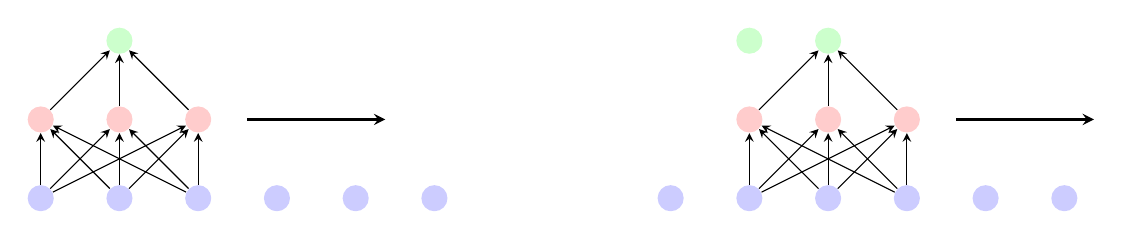
\begin{tikzpicture}
    %%%% PRODUCING FIRST OUTPUT %%%% 
    % Conv filter
    \node (cperc0) [conv_perc] {};
    \node (cperc1) [conv_perc, right of=cperc0] {};
    \node (cperc2) [conv_perc, right of=cperc1] {};
    % Empty nodes for arrow showing filter movement
    \node (empty_node1) [empty, right of=cperc2, xshift=-0.5cm] {};
    \node (empty_node2) [empty, right of=empty_node1, xshift=1cm] {};
    % Layer below conv
    \node (perc0) [reg_perc, below of=cperc0] {};
    \node (perc1) [reg_perc, below of=cperc1] {};
    \node (perc2) [reg_perc, below of=cperc2] {};
    \node (perc3) [reg_perc, right of=perc2] {};
    \node (perc4) [reg_perc, right of=perc3] {};
    \node (perc5) [reg_perc, right of=perc4] {};
    % Output of conv filter
    \node (output) [output, above of=cperc1] {};
    %% Arrows
    % conv_perc0
    \draw [arrow] (perc0) -- (cperc0);
    \draw [arrow] (perc1) -- (cperc0);
    \draw [arrow] (perc2) -- (cperc0);
    % conv_perc1
    \draw [arrow] (perc0) -- (cperc1);
    \draw [arrow] (perc1) -- (cperc1);
    \draw [arrow] (perc2) -- (cperc1);
    % conv_perc2
    \draw [arrow] (perc0) -- (cperc2);
    \draw [arrow] (perc1) -- (cperc2);
    \draw [arrow] (perc2) -- (cperc2);
    % Output
    \draw [arrow] (cperc0) -- (output);
    \draw [arrow] (cperc1) -- (output);
    \draw [arrow] (cperc2) -- (output);
    % Arrow for illustrating filter movement
    \draw [thick_arrow] (empty_node1) -- (empty_node2);
    
    %%%% PRODUCING SECOND OUTPUT %%%%
    % Layer below conv
    \node (perc10) [reg_perc, right of=perc5, xshift=2cm] {};
    \node (perc11) [reg_perc, right of=perc10] {};
    \node (perc12) [reg_perc, right of=perc11] {};
    \node (perc13) [reg_perc, right of=perc12] {};
    \node (perc14) [reg_perc, right of=perc13] {};
    \node (perc15) [reg_perc, right of=perc14] {};
    % Conv filter
    \node (cperc10) [conv_perc, above of=perc11] {};
    \node (cperc11) [conv_perc, above of=perc12] {};
    \node (cperc12) [conv_perc, above of=perc13] {};
    % Output
    \node (output11) [output, above of=cperc11] {};
    \node (output10) [output, left of=output11] {};
    % Empty nodes for arrow showing filter movement
    \node (empty_node11) [empty, right of=cperc12, xshift=-0.5cm] {};
    \node (empty_node12) [empty, right of=empty_node11, xshift=1cm] {};
    %% Arrows
    % conv_perc0
    \draw [arrow] (perc11) -- (cperc10);
    \draw [arrow] (perc12) -- (cperc10);
    \draw [arrow] (perc13) -- (cperc10);
    % conv_perc1
    \draw [arrow] (perc11) -- (cperc11);
    \draw [arrow] (perc12) -- (cperc11);
    \draw [arrow] (perc13) -- (cperc11);
    % conv_perc2
    \draw [arrow] (perc11) -- (cperc12);
    \draw [arrow] (perc12) -- (cperc12);
    \draw [arrow] (perc13) -- (cperc12);
    % Output
    \draw [arrow] (cperc10) -- (output11);
    \draw [arrow] (cperc11) -- (output11);
    \draw [arrow] (cperc12) -- (output11);
    % Arrow for illustrating filter movement
    \draw [thick_arrow] (empty_node11) -- (empty_node12);
\end{tikzpicture}
    \caption{An illustration of how a one-dimensional convolutional layer works. The blue circles represent the input to the convolutional layer, the red circles represent units that make up the convolutional layer, the green circles represent the output of the convolutional layer, the thin arrows between units represent the weighted sum, and the thick arrow represents the sliding of the filter over the input.}
    \label{fig:conv}
\end{figure}

\subsection{Recurrent Layers}
An attribute that was long sought after was the ability of an \acrshort{ann} to detect time-dependent relations between the input. Especially in the fields of time-series analysis, natural language processing, and video analysis. To address this problem, special perceptrons with ''memory'' were introduced, and layers of these perceptrons are called \textit{recurrent layers}. The way that the memory attribute was added to recurrent units was by introducing a feedback loop such that the past output was added to the weighted sum of inputs with a separate weight, as illustrated in figure \ref{fig:lstm}. One implementation of this type of unit is called the \acrfull{lstm} unit. It works by giving a memory unit to a perceptron, which has three \textit{gates} that regulate the flow of information within the unit: write, read, and flush. The write gate controls to which extent new inputs are allowed into the unit, the write gate controls the weighting that the old values in the unit are given, when calculating the output and the flush gate controls how long a particular value is allowed to remain in the unit \cite{lstm_wikipedia}. \acrshort{ann} that apply recurrent layers and dense layers are called a \acrfull{rnn}. The name "deep neural network" is used for architectures that are "deep", meaning that they consist of many layers. There is no formal limit of how many layers an architecture must have before it is considered deep, so \acrfull{ann} is the nomenclature that will be used for the model in this work. 

\begin{figure}[H]
    \centering
    \tikzstyle{init} = [pin edge={to-,thin,black}]
\tikzstyle{circ} = [circle, minimum size=1cm, text centered, draw=black, fill=blue!20]
\tikzstyle{arrow} = [thin,->,>=stealth]

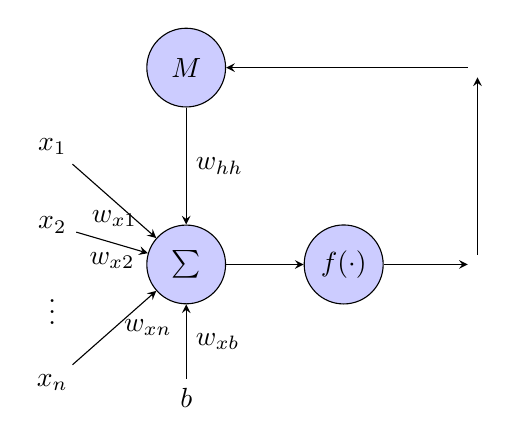
\begin{tikzpicture}
    % Perceptron
    \node (x1)    [init] {$x_1$};
    \node (x2)    [init, below of=x1] {$x_2$};
    \node (vdots) [init, below of=x2] {$\vdots$};
    \node (xn)    [init, below of=vdots] {$x_n$};
    
    \node (sum)    [circ, right of=x2, xshift=0.7cm, yshift=-5mm] {$\sum$};
    \node (b)      [init, below of=sum, yshift=-0.7cm] {$b$};
    \node (obj)    [circ, right of=sum, xshift=1cm] {$f(\cdot)$};
    \node (output) [init, right of=obj, xshift=0.7cm] {};
    \node (empty1) [init, above of=output, yshift=1.5cm] {};
    \node (lstm)   [circ, above of=sum, yshift=1.5cm] {$M$};
    
    \draw [arrow] (x1) --node[anchor=north] {$w_{x1}$} (sum);
    \draw [arrow] (x2) --node[anchor=north] {$w_{x2}$} (sum);
    \draw [arrow] (xn) --node[anchor=west] {$w_{xn}$} (sum);
    \draw [arrow] (b) --node[anchor=west] {$w_{xb}$} (sum);
    \draw [arrow] (sum) -- (obj);
    \draw [arrow] (obj) -- (output);
    \draw [arrow] (output) -- (empty1);
    \draw [arrow] (empty1) -- (lstm);
    \draw [arrow] (lstm) --node[anchor=west] {$w_{hh}$} (sum);
\end{tikzpicture}
    \caption{An simplified illustration of the memory in an LSTM unit.}
    \label{fig:lstm}
\end{figure}

\subsection{Underfitting and Overfitting}
When training an \acrshort{ann} for deployment, it is common to divide the data one has at hand into a training set, a validation set, and a test set. The training and validation sets are used during training, and the test set is used after training to benchmark the model. When an \acrshort{ann} is trained, \acrshort{sgd} with back-propagation is performed on the training set, simultaneously the model is evaluated on an independent validation set. This is done to determine whether the model is \textit{overfitting} on the training set. Overfitting is described as when a model performs well on the training set, but underperforms on the validation and test set. This is common among complex \acrshort{ann} architectures, and can be a sign that the architecture applied is too complex for the dataset. \textit{Underfitting} is said to occur when the accuracy of the model on the training set is lower than to be expected, this is often a sign that architecture of the \acrshort{ann} is too simple, and can be expanded.

\section{Evaluation Metrics} \label{sec:eval_metrics}
In medicine one often assesses a test for a specific disease in terms of how many \acrfull{tp}, \acrfull{tn}, \acrfull{fp} and \acrfull{fn} the test attains. The meaning of these terms is illustrated in table \ref{tab:ttpnffpn}. If a patient is sick and the test classifies the patient as sick, this result is regarded as a \acrlong{tp}. If a patient is sick and is classified healthy by the test, it is regarded as a \acrlong{fn}. If a patient is healthy and is classified healthy by the test, it is regarded as a \acrlong{tn}. Finally, if a patient is healthy and is classified as sick, this is regarded as a \acrlong{fp}. These metrics are also used frequently for assessing the performance of binary classifiers. They can be used on multi-class classifiers as well, but then one would have to calculate a set of metrics for each class. For classifiers the aim is always to maximize the number of \acrshort{tp}, and \acrshort{tn} and minimize the number of \acrshort{fp}, and \acrshort{fn}. The common metric accuracy can be defined in terms of these metrics as $(\mathrm{TP} + \mathrm{TN}) / (\mathrm{TP} + \mathrm{TN} + \mathrm{FP} + \mathrm{FN})$.

\begin{table*}
    \centering
    \ra{1.3}
    \begin{tabular}{c|c|c|}
        \toprule
                             & Patient is sick & Patient is healthy \\
        \midrule
        Patient tests sick   & \acrshort{tp}   & \acrshort{fp} \\
        \midrule
        Patiet tests healthy & \acrshort{fn}   & \acrshort{tn} \\
        \bottomrule
    \end{tabular}
    \caption{Illustration of how the metrics \acrshort{tp}, \acrshort{tn}, \acrfull{fp} and \acrfull{fn} are defined.}
    \label{tab:ttpnffpn}
\end{table*}

\subsection{Sensitivity, Specificity, and Diagnostic Odds Ratio}
Usually, it can be helpful to combine the four metrics shown in table \ref{tab:ttpnffpn} into two more compact metrics known as sensitivity (true positive rate) and specificity (true negative rate), which are defined in equation \eqref{eq:sens_spec}. Sensitivity is defined as the number of positive cases correctly classified, divided by the total number of positive cases in the dataset. Similarily specificity is defined as the total number of negatives correctly classified divided by the total number of negatives in the dataset. If a dataset does not have an even distribution of positives or negatives, the accuracy can be inflated if a model is only able to perform well at classifying one class. Analyzing the sensitivity and specificity allows one to get a better understanding of how well a model works at detecting each category. As with accuracy, sensitivity and specificity can range from zero to one.

\begin{equation}
    \begin{split}
        \mathrm{Sensitivity} &= \frac{\mathrm{TP}}{\mathrm{TP} + \mathrm{FN}} \\
        \mathrm{Specificity} &= \frac{\mathrm{TN}}{\mathrm{TN} + \mathrm{FP}}
    \end{split}
    \label{eq:sens_spec}
\end{equation}

A third metric that is useful when comparing multiple classifiers is known as \acrfull{dor}. It is defined by equation \eqref{eq:dor}. What one can see quickly is that the value of the \acrshort{dor} is unbounded, in contrast to the accuracy, sensitivity, and specificity metrics. This is both a blessing and a curse. The advantage of this is that differences that may seem very small in terms of accuracy, sensitivity, and specificity become very evident in the \acrshort{dor}. The disadvantage is that the metric is undefined if either \acrshort{fp} or \acrshort{fn} are zero. An advantage of the \acrshort{dor} is that it takes both \acrshort{tp} and \acrshort{tn} into account, whereas other metrics such as the F1-score does not take \acrshort{tn} into account. 

\begin{equation}
    \mathrm{DOR} = \frac{\mathrm{TP}\times\mathrm{TN}}{\mathrm{FP}\times\mathrm{FN}}
    \label{eq:dor}
\end{equation}

\subsection{Adjusted Rand Index}
The \acrfull{ari} is a version of the Rand Index, that is ''adjusted for chance''. The Rand Index applied in binary classification problems is equivalent to accuracy \cite{ari_wikipedia}. However, it might be more helpful to view the \acrshort{ari} as a measure of how much the distribution of two groupings\footnote{Groupings refers to a segregation of a dataset into distinct non-overlapping groups with separate labels. An example of a grouping can be a set of cluster assignments.} of a dataset overlap. Given that one has a dataset $X$ with $n$ objects $X = \{x_1, x_2, ..., x_n\}$, and two groupings of this dataset, $Y$ which has $p$ different labels, and $Z$ which has $q$ different labels. The first step of estimating the \acrshort{ari} is setting up a contingency table shown in table \ref{tab:cont} \cite{ari_wikipedia}. Here entry $n_{ij}$ is the number of data objects that have label $Z_i$ in the $Z$-grouping and label $Y_j$ in the $Y$-grouping, $a_i$ is the number of data objects with the $Z_i$ label, and $b_j$ is the number of data objects with the $Y_j$ label. The \acrshort{ari} is then calculated according to equation \eqref{eq:ari}

\begin{table*}
    \centering
    \ra{1.3}
    \begin{tabular}{c|cccc|c}
        \toprule
                 &  $Y_1$   &  $Y_2$   & $\hdots$ & $Y_p$    & $\sum$ \\
        \midrule
        $Z_1$    & $n_{11}$ & $n_{12}$ & $\hdots$ & $n_{1p}$ & $a_1$ \\
        \midrule
        $Z_2$    & $n_{21}$ & $n_{22}$ & $\hdots$ & $n_{2p}$ & $a_2$ \\
        \midrule
        $\vdots$ & $\vdots$ & $\vdots$ & $\ddots$ & $\vdots$ & $\vdots$ \\
        \midrule
        $Z_q$    & $n_{q1}$ & $n_{q2}$ & $\hdots$ & $n_{qp}$ & $a_p$ \\
        \midrule
        $\sum$   &  $b_1$   &  $b_2$   & $\hdots$ &  $b_q$   &
    \end{tabular}
    \caption{Contingency table used to calculate \acrshort{ari}. Inspired by the table used by \cite{ari_wikipedia}}
    \label{tab:cont}
\end{table*}

\begin{equation}
    \mathrm{ARI} = \frac{\sum_{ij} \binom{n_{ij}}{2} - \frac{\left [ \sum_i \binom{a_i}{2} \sum_j \binom{b_j}{2} \right ]}{\binom{n}{2}} }{0.5\left [ \sum_i \binom{a_i}{2} + \sum_j \binom{b_j}{2} \right ] - \frac{\left [ \sum_i \binom{a_i}{2} \sum_j \binom{b_j}{2} \right ]}{\binom{n}{2}}}
    \label{eq:ari}
\end{equation}

\section{Chapter Summary}

In section \ref{sec:theory_clust} it is specified that whole-series \acrshort{tsc} is what will be used in this work. The different approaches and objectives of \acrshort{tsc} are discussed. In section \ref{sec:theory_diss}, the different dissimilarity metrics that are to be used in the clustering models are presented, Euclidean distance and \acrshort{dtw}. The hierarchical agglomerative clustering algorithm is introduced as a hard clustering algorithm that takes a dissimilarity matrix as input and yields a hierarchy of clusters as output called a dendrogram. The different linkage criteria used in this are presented, and the section ends by explaining the term ''curse of dimensionality''. \bigskip

In section \ref{sec:ann} many aspects of \acrshort{ann} were discussed. The basic building blocks, perceptrons were presented and how they consist of weighted sums and activation functions. Section \ref{sec:nn_training} explained how \acrshort{ann} are trained with feed-forward computation, and \acrshort{sgd} with back-propagation. Two special layers were presented, convolutional layers and recurrent layers that serve their specific purpose in an \acrshort{ann} architecture. The section ends with discussing the two common issues of underfitting and overfitting. \bigskip
 
The chapter ends with section \ref{sec:eval_metrics} which explains the different evaluation metrics used in this work: Accuracy, sensitivity, specificity, \acrshort{dor} and \acrshort{ari}.
